\chapter{Fundamentos teóricos}

Este capítulo tiene el propósito de presentar y describir los fundamentos teóricos que sustentan los métodos 
utilizados en el trabajo, además de justificar su importancia para abordar los problemas planteados.

% ------------------------------------------------------------------------------------------------------------
% MACHINE LEARNING -------------------------------------------------------------------------------------------
% ------------------------------------------------------------------------------------------------------------

\section{Machine Learning}

Frente a la idea de intentar crear un programa que simulara directamente el comportamiento inteligente de una ``mente adulta'', Alan Turing ya vaticinó un enfoque alternativo \cite{turing1950}: que las máquinas pudieran aprender como lo hace un niño, mediante un ``proceso educativo'' con el cual se logra alcanzar progresivamente una ``mente adulta'', obteniendo así comportamientos inteligentes complejos.

En los años 50, surgió el concepto de \textit{machine learning} (\acrshort{ML}) ---o aprendizaje automático en español---, popularizado por Arthur L. Samuel \cite{samuel1959}, para designar una rama marginal de la \acrshort{IA}, centrada en el desarrollo de modelos y algoritmos que permitiesen a las computadoras imitar la forma en la que los humanos aprenden, realizar tareas autónomas y mejorar su rendimiento a través de la experiencia y exposición a más datos. De esta forma, estos modelos podrían realizar predicciones o tomar decisiones sin ser programados para cada caso.

En las décadas de 1960, 1970 y 1980, surgieron algoritmos fundamentales como el perceptrón \cite{mcculloch1943,rosenblatt1958} o los árboles de decisión \cite{quinlan1986}, que sentaron los cimientos teóricos para el desarrollo posterior de técnicas más complejas. Sin embargo, el progreso fue lento debido a las limitaciones computacionales y el gran escepticismo académico. 

Los años 90 y 2000 marcaron un punto de inflexión para el \acrshort{ML}, gracias a los avances teóricos, el mayor poder computacional y la disponibilidad de grandes volúmenes de datos. De 2010 en adelante, la evolución del \acrshort{ML} ha sido exponencial, marcada por la consolidación del \textit{deep learning}, la escalabilidad masiva y su integración en numerosas aplicaciones: de visión por computador, reconocimiento de lenguaje natural, robótica, diagnóstico médico y forense, finanzas o recomendación de contenidos, entre otros. De esta forma, el \acrshort{ML} se ha convertido en un campo tan amplio y exitoso que ahora ``eclipsa'' al resto de campos de la \acrshort{IA} \cite{domingos2015}.

El \acrshort{ML} diferencia tres tipos de aprendizaje en base a tres tipos de retroalimentación \cite{rusell2021}: 

\begin{itemize}
    
    \item \textbf{Aprendizaje supervisado}, en el que el agente (refiriéndose con este al modelo de \acrshort{ML} y su algoritmo de aprendizaje) observa ejemplos de pares entrada-salida y aprende la función que mejor mapea las entradas (\textit{inputs}) a las salidas (\textit{outputs}) correspondientes. El objetivo es generalizar este aprendizaje para hacer predicciones precisas sobre datos nuevos y no vistos \cite{bishop2006}.

    \item \textbf{Aprendizaje por refuerzo}, en el que los datos de entrenamiento no contienen salida objetivo, sino que contiene posibles resultados junto con medidas de calidad de dicho resultado, es decir, una función de evaluación del estado. En este tipo de aprendizaje, el agente toma decisiones en un entorno y recibe recompensas o penalizaciones por las acciones que realiza, ajustando su comportamiento mediante prueba y error, maximizando la recompensa acumulada en el tiempo \cite{alpaydin2010}.

    \item \textbf{Aprendizaje no supervisado}, en el que el agente tampoco dispone de valores de salida, solo de entrada \cite{bishop2006}, y los objetivos pueden ser muy variados, centrándose en descubrir patrones, estructuras o relaciones ocultas en los datos. A diferencia de los otros enfoques, aquí no hay una ``respuesta correcta'' predefinida, sino que el modelo debe inferir conocimiento directamente desde la distribución de los datos.

\end{itemize}

Este trabajo se centrará en el aprendizaje supervisado, pues es este tipo de aprendizaje el empleado en los problemas de clasificación y regresión que aplicaremos en el ámbito de la antropología forense.

El objetivo en el aprendizaje supervisado es establecer una hipótesis que se ajuste de forma óptima a los ejemplos futuros. Para ello, se presupone que los ejemplos futuros mostrarán un comportamiento similar a los pasados. Bajo este supuesto, el ajuste óptimo de un modelo es, por tanto, la hipótesis que minimiza la tasa de error del problema \cite{rusell2021}.


% Retos en el aprendizaje supervisado


% No importa el formato de entrada



% ------------------------------------------------------------------------------------------------------------

% En el \textbf{aprendizaje supervisado} \cite{bishop2006}, el agente (refiriéndose con este al 
% modelo de ML y su algoritmo de aprendizaje) observa ejemplos de pares entrada-salida y aprende
% la función que mejor mapea las entradas (inputs) a las salidas (outputs) correspondientes. El 
% objetivo es generalizar este aprendizaje para hacer predicciones precisas sobre datos nuevos y 
% no vistos.

% Hay dos principales tipos de problemas de aprendizaje supervisado: 

% \begin{itemize}
%     \item la \textit{clasificación} para cuando el valor de salida es una etiqueta categórica, y
%     \item la \textit{regresión} cuando el valor de salida es un valor continuo.
% \end{itemize}

% % ----------------------------------------------------------------------------------------------------------

% En cambio, en el \textbf{aprendizaje por refuerzo}, los datos de entrenamiento no contienen 
% salida objetivo, sino que contiene posibles resultados junto con medidas de calidad de dicho 
% resultado, es decir, una función de evaluación del estado. En este tipo de aprendizaje, el 
% agente toma decisiones en un entorno y recibe recompensas o penalizaciones por las acciones 
% que realiza, ajustando su comportamiento mediante prueba y error, maximizando la recompensa 
% acumulada en el tiempo \cite{alpaydin2010}.  

% De esta forma, el algoritmo no aprende a dar una acción/salida a partir de un input, sino que 
% desarrolla una política que determina la mejor acción a tomar en cada estado del entorno, con 
% el objetivo de maximizar la recompensa acumulada a largo plazo.

% Esta aproximación es clave en aplicaciones como juegos, robótica, optimización de recursos y 
% sistemas conversacionales (ChatAI), donde las decisiones secuenciales y la interacción 
% dinámica con el entorno son fundamentales.

% % ----------------------------------------------------------------------------------------------------------

% Y, por último, en el \textbf{aprendizaje no supervisado}, el agente tampoco dispone de valores 
% de salida, solo de entrada \cite{bishop2006}, y los objetivos pueden ser muy variados, 
% centrándose en descubrir patrones, estructuras o relaciones ocultas en los datos. 

% A diferencia de los otros enfoques, aquí no hay una "respuesta correcta" predefinida, sino que 
% el modelo debe inferir conocimiento directamente desde la distribución de los datos.

% Algunos problemas clásicos de este tipo de aprendizaje son: 

% \begin{itemize}

%     \item El \textit{clustering} o agrupamiento, donde el objetivo es encontrar clústeres o 
%     agrupaciones del input. Esto puede ser útil, por ejemplo, para una empresa que quiera 
%     segmentar sus clientes, o para identificar patrones en datos genéticos sin etiquetar.
    
%     \item La \textit{detección de anomalías} (\textit{outlier detection} en inglés), que 
%     consiste en encontrar instancias atípicas o inusuales en los datos. Sus aplicaciones 
%     incluyen: identificación de fraudes en transacciones bancarias, fallos en equipos 
%     industriales o identificación de ciberataques.

%     \item La \textit{reducción de dimensionalidad}, que trata de reducir el número de 
%     variables manteniendo la mayor información posible. Esto es útil para visualizar datos 
%     complejos o mejorar la eficiencia de algoritmos (p.ej., transformaciones PCA y t-SNE).

%     \item El \textit{aprendizaje de representaciones} (como los \textit{autoencoders}), 
%     donde el modelo busca capturar características latentes de los datos de manera eficiente. 
%     La compresión de archivos o la reducción de ruido en imágenes son algunos ejemplos de 
%     aplicaciones. 

% \end{itemize}



% ------------------------------------------------------------------------------------------------------------

\subsection{Problemas de regresión}

Como se ha mencionado antes, la regresión es un tipo de problema clásico en el aprendizaje supervisado, y consiste en predecir el valor de una o más \textbf{variables continuas} objetivo a partir de unos datos de entrada \cite{bishop2006}, utilizando un modelo entrenado con ejemplos ya con valores conocidos.

Matemáticamente, este proceso implica modelar la relación entre la variable dependiente $Y$ y las variables independientes $X$, de modo que se pueda predecir o explicar el comportamiento de $Y$ en función de los valores de $X$. El modelo aprende una función de predicción $f$ que, dado un nuevo ejemplo $i$ con características $X_i$, genera una estimación $\hat{Y_i}$:

$$
f(X_i) = f(X_{i0}, X_{i1}, \dots, X_{in}) = \hat{Y_i} = Y_i + \varepsilon_i
$$

donde 

\begin{itemize}
    \item $X_{i0},X_{i1}, \dots, X_{in}$ son las características o atributos del ejemplo $i$,
    \item $Y_i$ es el valor real de la variable objetivo para ese ejemplo,
    \item $\hat{Y_i}$ es la predicción generada por el modelo, y
    \item $\varepsilon_i$ representa el error o residuo%
    \footnote{
        A pesar de que en la literatura más especializada ---que veremos a continuación---, los términos 
        ``error'' y ``residuo'' se distinguen. 
    }, 
    es decir, la diferencia entre la predicción y el valor real.
    Este término captura factores aleatorios o imprecisiones que el modelo no logra explicar perfectamente.
\end{itemize}

El análisis y la evaluación estadística del error son fundamentales para valorar la utilidad práctica del 
modelo y optimizar su capacidad predictiva mediante técnicas de ajuste y validación.

% ------------------------------------------------------------------------------------------------------------

\subsection{Problemas de clasificación}

En cambio, en los problemas de clasificación, los valores de salida son categóricos, denominados más comúnmente como \textbf{clases}, y a cada valor individual asignado a una instancia de datos se le conoce como \textbf{etiqueta} (\textit{label} en inglés).

Existen multitud de variante de clasificación, que pueden diferenciarse según diversos criterios:

\begin{itemize}
    \item En base a la cardinalidad de las clases de salida: \textbf{clasificación binaria o multiclase}, según si existen dos clases posibles o más de dos, respectivamente.

    \item En base al número de etiquetas asignadas a cada instancia: \textbf{clasificación con etiqueta única o multietiqueta}, según si cada instancia pertenece a una sola clase o a varias de forma simultánea.

    \item En base a la certeza de la asignación de clases: \textbf{clasificación con etiqueta precisa o difusa}, donde en el primer caso la asignación a una clase es determinista, y en el segundo caso se permite una pertenencia parcial a varias clases, con distinto grados de afinidad.
    
\end{itemize}

No obstante, la mayoría de los problemas estudiados en la literatura de \acrshort{ML}, y concretamente en antropología forense, corresponden a clasificación binaria o multiclase, con etiquetas únicas y asignación precisa \cite{bishop2006}, que será el tipo de clasificación en el que nos centraremos. La cardinalidad de las clases tiene implicaciones significativas en el diseño del modelo y la evaluación de su desempeño:

\begin{itemize}

    \item \textbf{Clasificación binaria}, que es aquella en la que existen únicamente dos clases posibles para la variable objetivo, siendo común en problemas donde se desea discriminar entre dos estados mutuamente excluyentes (p.ej., ``positivo'' vs. ``negativo'', ``spam'' vs. ``no spam'', ``fraude'' vs. ``no fraude'').
    
    Se suele denominar a una de las clases como ``positiva'' y a otra como ``negativa'' para facilitar la interpretación de métricas como la precisión, la sensibilidad o la especifidad, si bien no tiene por qué existir una connotación valorativa entre ambas clases.
    
    \item \textbf{Clasificación multiclase}: en este caso, la variable objetivo puede tomar más de dos valores posibles, pertenecientes a un conjunto finito. Un ejemplo de problema clásico es el de clasificar dígitos manuscritos (0-9).

\end{itemize}

En este tipo de problemas, el error ocurre cuando no se acierta al predecir la clase del ejemplo.

% Tanto en clasificación binaria como multiclase, un problema común es el desequilibrio de clases, donde una 
% clase tiene muchos más ejemplos que otra. Esto afecta el entrenamiento del modelo, ya que puede sesgarse 
% hacia la clase mayoritaria, ya que el modelo





% ------------------------------------------------------------------------------------------------------------
% ENSEMBLE LEARNING ------------------------------------------------------------------------------------------
% ------------------------------------------------------------------------------------------------------------

% \section{Ensemble Learning}

% El \textbf{aprendizaje por conjuntos (\textit{ensemble learning})} es una familia de técnicas de ML que 
% combina múltiples modelos de aprendizaje automático ---denominados \textbf{modelos base}--- para obtener un 
% modelo final con un mejor desempeño que los modelos base por separado.

% \subsection{Bagging}


% \subsection{Boosting}


% \subsection{Stacking}


% ------------------------------------------------------------------------------------------------------------
% DEEP LEARNING ----------------------------------------------------------------------------------------------
% ------------------------------------------------------------------------------------------------------------

\section{Deep Learning}

El \textbf{aprendizaje profundo (\textit{deep learning}, \acrshort{DL})} es una familia de técnicas de \acrshort{ML} que utilizan múltiples capas de procesamiento para aprender representaciones de datos con varios niveles de abstracción \cite{lecun2015}. Las redes neuronales han demostrado ser especialmente eficaces para este propósito, al permitir la composición jerárquica de características que capturan patrones cada vez más complejos en los datos. Estas tienen su origen en el intento de modelar las redes de neuronas del cerebro humano \cite{mcculloch1943}. Se requirió de numerosas contribuciones teóricas ---como el perceptrón \cite{rosenblatt1958} o el algoritmo de \textit{backpropagation} \cite{rumelhart1986,werbos1994}, entre otras---, disponibilidad de datos estandarizados y un gran aumento en la capacidad computacional para poder escalar estar redes y obtener resultados sorprendentes en tareas complejas.

Las \textbf{redes neuronales profundas (\textit{deep neural networks}, \acrshort{DNN})} destacan por su capacidad para 
aprender representaciones jerárquicas: cada capa extrae características progresivamente más abstractas 
\cite{lecun2015}, desde líneas en imágenes hasta formas geométricas complejas, objetos completos e incluso 
escenas compuestas.
Esta propiedad las hace excepcionalmente versátiles, ya que procesan datos de muy diversa naturaleza ---datos 
tabulares, imágenes, audio, texto o señales temporales---, dados que ellas mismas aprenden los procesos de 
extracción de características de estos, hasta ahora realizados ``a mano'' (mediante procesos diseñados por la 
ingeniería de características)%
\footnote{
    Este enfoque se denomina aprendizaje extremo a extremo (\textit{end-to-end learning}), en el cual tanto la 
    extracción de características como la clasificación son parte de un modelo integral que se entrena de 
    manera conjunta, optimizando todos los componentes del sistema en un mismo proceso \cite{rusell2021}.
}
\cite{rusell2021}. 
Gracias a ello, las \acrshort{DNN} han alcanzado rendimientos sobresalientes en dominios como visión por computador 
(clasificación de imágenes, detección de objetos, segmentación) o procesamiento de lenguaje natural 
(traducción, generación de texto) \cite{redhat2024DeepLearningDefinition}.
No obstante, su eficacia depende críticamente de grandes volúmenes de datos y recursos computacionales, lo que 
ha impulsado técnicas como el \textit{transfer learning} y modelos eficientes para democratizar su uso.


\subsection{El perceptrón multicapa}

El \textbf{perceptrón multicapa (\textit{multilayer perceptron}, \acrshort{MLP})} forma la base del \textit{deep learning}. Su diseño ---con capas ocultas, funciones de activación no lineales y entrenamiento  mediante \textit{backpropagation}--- sentó las bases conceptuales para arquitecturas más complejas, como las redes neuronales convolucionales o los \textit{transformers} \cite{murphy2022}. El \acrshort{MLP} sigue siendo un referente teórico y la expresión más simple de cómo el aprendizaje jerárquico puede capturar patrones en los datos. 

Cada nodo en la red es denominado \textbf{unidad o neurona artificial}. Siguiendo el diseño propuesto en \cite{mcculloch1943,rosenblatt1958}, cada unidad recibe señales de entrada ---que o bien son las características de los datos o bien las salidas de las unidades de la anterior capa---, realiza una suma ponderada de estas con los pesos entrenables de cada conexión ---más un término independiente o sesgo, también entrenable---, aplica una función no lineal sobre esta para producir una salida que propaga a las unidades de la siguiente capa (véase la Figura \ref{fig:neuron_MLP}).

Matemáticamente, la operación de una unidad artificial se expresaría como:

$$
y = f \left( \sum_{i=1}^n{w_ix_i+b} \right)
$$

donde $x_i$ son las entradas, $w_i$ son los pesos entrenables ($w_0$ el sesgo)%
\footnote{
    El sesgo se considera un peso, puesto que, en la implementación, son un peso más conectado a una unidad de sesgo con valor constante unitario (1).
}
, y $f$ es la función de activación.

\begin{figure}[htbp]
    \centering
    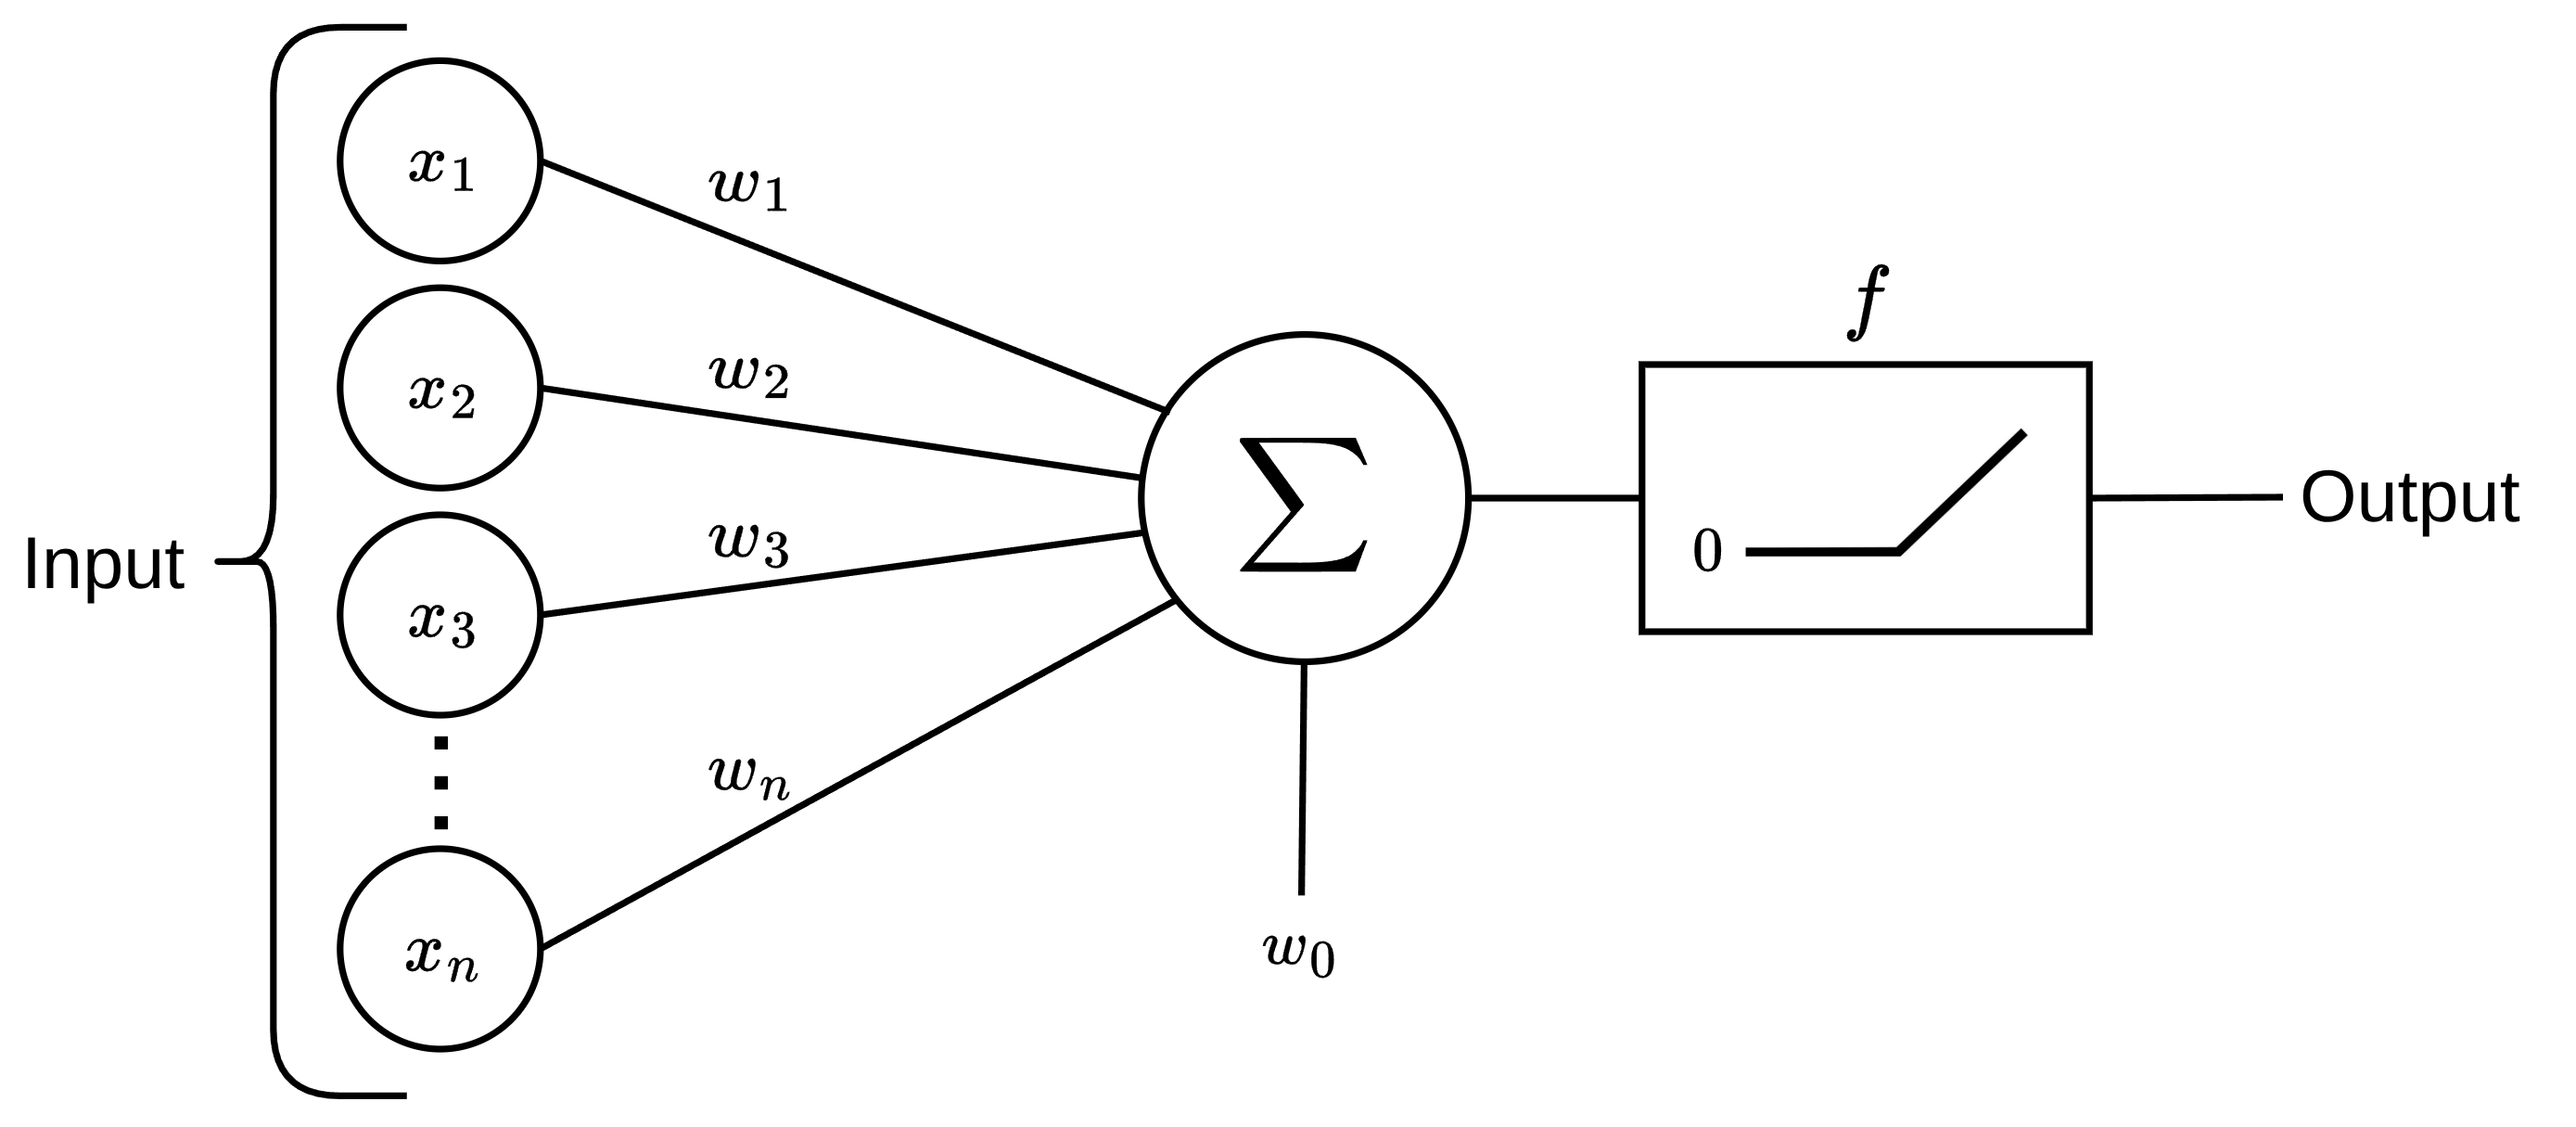
\includegraphics[width=0.95\textwidth]{capitulos/cap_02/imagenes/Neuron_perceptron.png}
    \caption[
        Esquema gráfico del funcionamiento de una unidad artificial de un perceptrón multicapa.
    ]{
        Esquema gráfico del funcionamiento de una unidad artificial de un perceptrón multicapa. 
        Adaptado de \cite{codeworld2022understandingMLDL}.
    } 
    \label{fig:neuron_MLP}
\end{figure}


Esta \textbf{función de activación} a la salida de la unidad es un componente esencial que introduce no 
linealidad en el modelo, permitiendo a la red aprender relaciones complejas en los datos%
\footnote{
    Sin ella, el \acrshort{MLP} se reduciría a una simple combinación lineal de las entradas, incapaz de
    representar jerarquías de características \cite{murphy2022}.
}.
Existe multitud de funciones de activación, como la sigmoide, la tangente hiperbólica o ReLu ---y sus 
múltiples variantes---, cada una con sus ventajas y limitaciones%
\footnote{
    Si bien, actualmente, ReLU y sus variantes (\textit{Leaky} ReLU, \textit{Parametric ReLU} o 
    \textit{Swish}) se han convertido en el estándar \textit{de facto} para las capas ocultas en \acrshort{DNN},
    por su eficiencia computacional, y su eficacia empírica \cite{vargas2021}.
}.

La arquitectura de un \acrshort{MLP} conecta estas unidades formando una red neuronal retroalimentada%
\footnote{
    Una red neuronal retroalimentada (\textit{feed-forward neural network}) es aquella en la que las 
    conexiones entre las unidades no forman un ciclo y, por tanto, la información solo se mueve en una 
    dirección: adelante.
},
que consta de tres partes (véase la Figura \ref{fig:neural_network}):

\begin{itemize}

    \item \textbf{Capa de entrada}, en las que el número de unidades debe coincidir con el formato de entrada de los datos, por ejemplo: en un problema con datos tabulares, debería haber una unidad por cada característica.
    
    \item \textbf{Capas ocultas}, donde se realizan las transformaciones no lineales de los datos. Es en estas donde el diseño puede variar en número de unidades y tipo de capas según la complejidad del problema y los datos.
    
    \item \textbf{Capa de salida}, que proporciona el resultado del modelo. Su forma depende del problema a 
    resolver: 
    
    \begin{itemize}
        
        \item en problemas de regresión, esta capa tendrá tantas unidades como variables a predecir ---sin 
        función de activación, ya que esto limitaría el rango de valores posibles---;
        
        \item en problemas de clasificación, esta capa tendrá una sola unidad ---generalmente, con activación 
        sigmoide--- en clasificación binaria, o múltiples unidades ---con activación 
        \textit{softmax}%
        \footnote{
            La activación \textit{softmax} no se aplica sobre la salida de una única unidad, sino que se 
            aplica sobre un vector de salidas de múltiples unidades, transformándolas en una distribución de 
            probabilidad, donde cada valor representa la probabilidad de pertenecer a una clase distinta y la 
            suma de todas las salidas es igual a 1.
        }
        --- en clasificación multiclase (véase la Figura \ref{fig:activation_func_classification}).
    \end{itemize}

\end{itemize}

\begin{figure}[htbp]
    \centering
    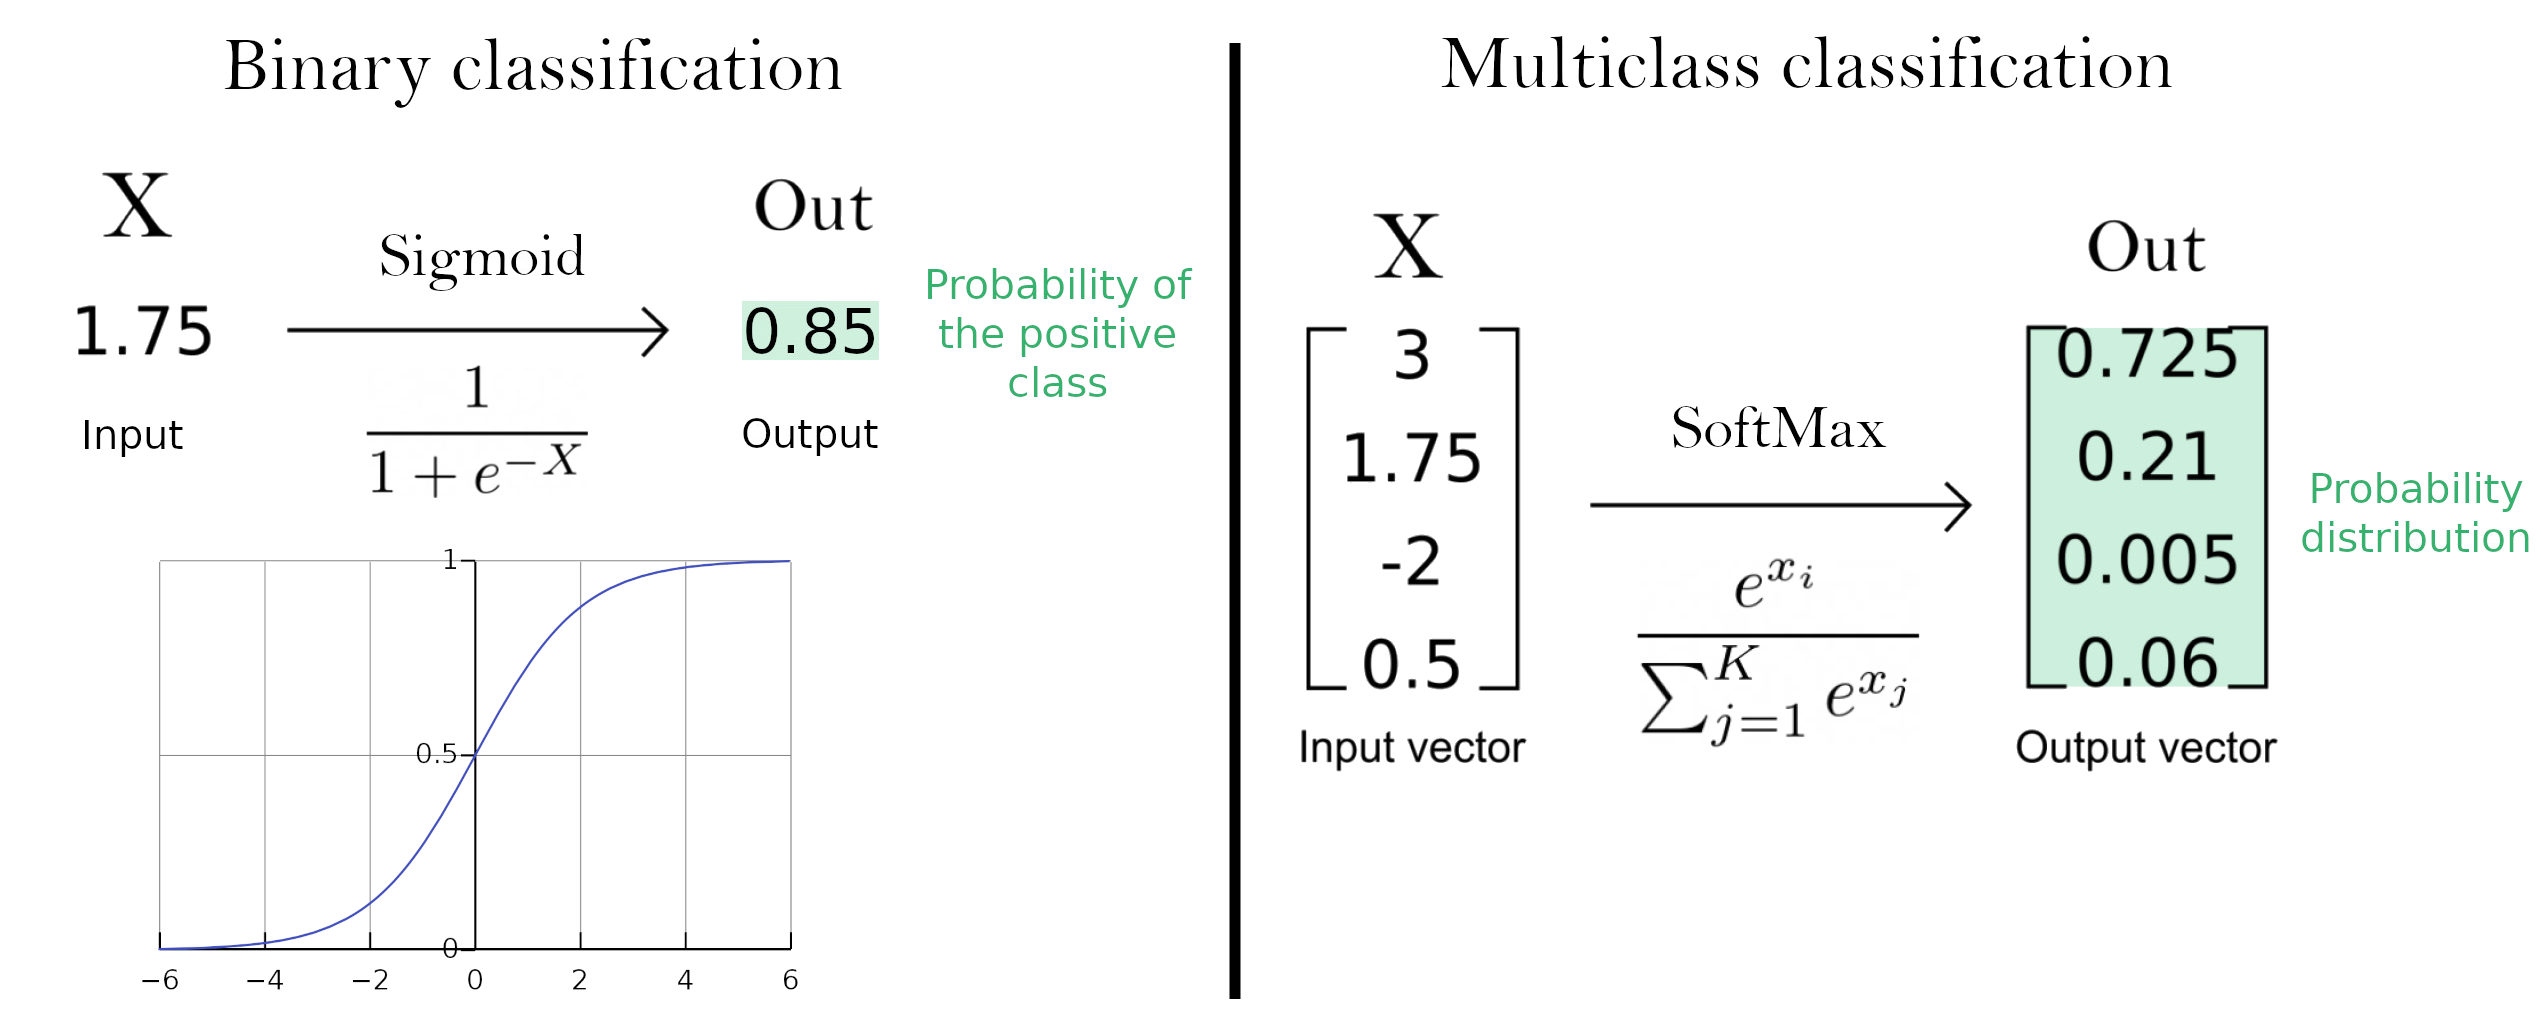
\includegraphics[width=\textwidth]{capitulos/cap_02/imagenes/ActivationFuncClassification.png}
    \caption[
        Esquema gráfico de obtención de probabilidades mediante sigmoide y \textit{softmax} en problemas de clasificación binaria y multiclase. 
    ]{
        Esquema gráfico de obtención de probabilidades mediante sigmoide y \textit{softmax} en problemas de clasificación binaria y multiclase, respectivamente. 
        Adaptado de \cite{furnieles2022sigmoidandsoftmax}.
    } 
    \label{fig:activation_func_classification}
\end{figure}

%Quitar X y Out, y subir lo de abajo

\begin{figure}[htbp]
    \centering
    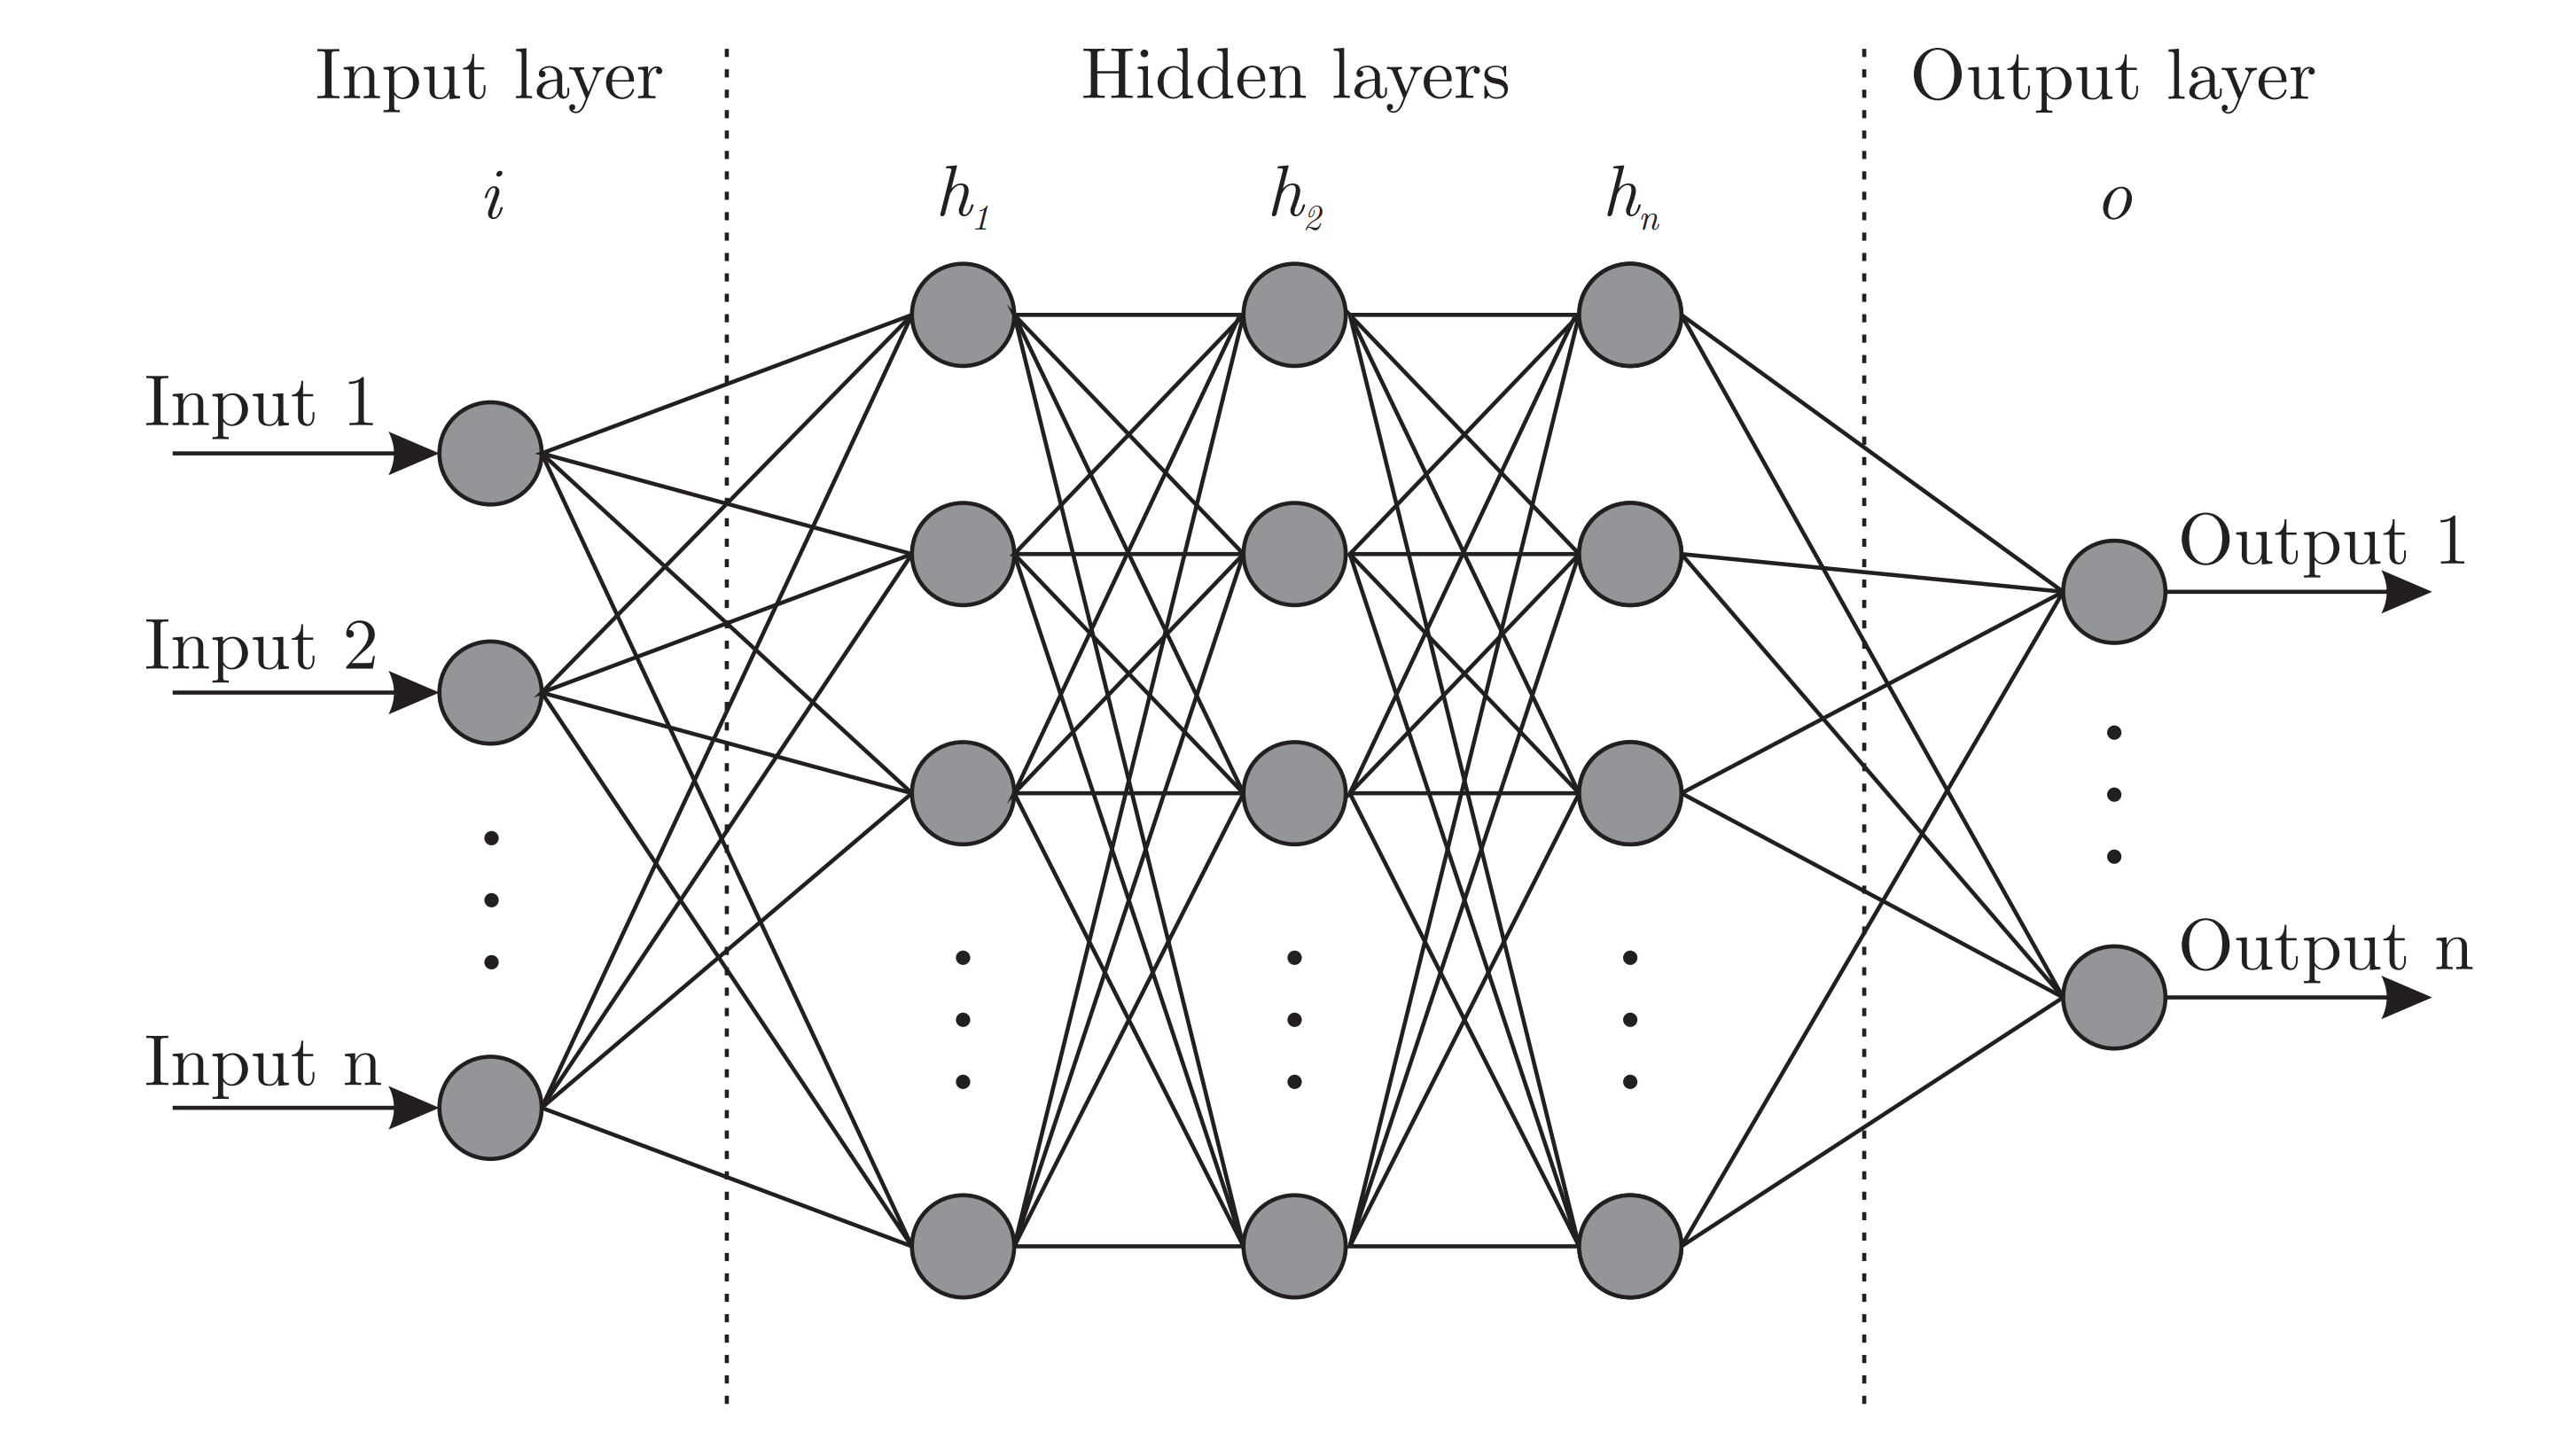
\includegraphics[width=0.95\textwidth]{capitulos/cap_02/imagenes/neural_network.png}
    \caption[
        Arquitectura simplificada de un MLP. 
    ]{
        Arquitectura simplificada de un \acrshort{MLP}. Recuperado de \cite{bre2017}.
    } 
    \label{fig:neural_network}
\end{figure}

% ------------------------------------------------------------------------------------------------------------

\subsection{Entrenamiento y validación de la red}

En el caso de las redes neuronales, el conjunto de datos suele dividirse en tres 
subconjuntos: entrenamiento, validación y prueba. A diferencia de métodos más tradicionales, no se utiliza 
validación cruzada, ya que entrenar redes profundas conlleva un elevado coste computacional.

Una vez hemos definido la arquitectura a emplear para resolver un problema, y definido los datos disponibles 
debemos entrenar la red con los datos de ejemplo. Este proceso implica ajustar los pesos del modelo para 
minimizar el error en las predicciones. 

El método de entrenamiento estándar en redes neuronales es el \textbf{algoritmo de retropropagación 
(\textit{backpropagation})}, que funciona en dos fases clave \cite{szeliski2010}:

\begin{itemize}

    \item \textbf{Propagación hacia adelante (\textit{forward pass})}: Los datos de entrada se procesan a 
    través de las capas de la red, generando una predicción. 

    \item \textbf{Propagación del error hacia atrás (\textit{backward pass})}: El error entre la 
    predicción y el valor real se calcula y se propaga hacia atrás en la red, ajustando los pesos mediante el 
    descenso de gradiente.
    
    Sin entrar en demasiado detalle, esto consiste en calcular el gradiente de la función de pérdida con           % Esto de "sin entrar en demasiado detalle" qué tal? 
    respecto a cada peso de la red, indicando cómo cada parámetro contribuye al error total. 
    A mayor aporte al error de un peso, más se ajustará ese peso. Así, el algoritmo priorizará modificar 
    significativamente los parámetros que más afectan al rendimiento de la red.
    
\end{itemize}

Este proceso explicado de manera vaga, tiene infinidad de detalles y variantes que influyen en su eficiencia y
eficacia:

\begin{itemize}

    \item El error obtenido entre la predicción y el valor real se calcula mediante la \textbf{función de 
    pérdida (\textit{loss function})}. Esta función cuantifica el error del modelo durante el entrenamiento, 
    midiendo la discrepancia entre las predicciones generadas y los valores o clases reales (\textit{ground 
    truth}).

    No se debe confundir con las métrica de evaluación de un modelo: aunque en algunos casos se pueden usar 
    métricas como funciones de pérdida y viceversa, las métricas destacan por ser fáciles de interpretar 
    y suele utilizarse más de una. En cambio, debe existir una única función de pérdida durante el 
    entrenamiento de una red neuronal, que debe cumplir tres requisitos clave:

    \begin{enumerate}

        \item Reflejar el objetivo del aprendizaje: Debe capturar adecuadamente qué significa ``éxito'' para 
        el modelo (p.ej., minimizar el error en regresión o maximizar la probabilidad de clasificación 
        correcta).

        \item Ser diferenciable: Es esencial para aplicar técnicas de descenso por gradiente, ya que el 
        optimizador necesita calcular derivadas.

        \item Ser eficiente computacionalmente: Dado que se evalúa en cada iteración del entrenamiento, su 
        cálculo debe ser rápido incluso con grandes volúmenes de datos.

    \end{enumerate}

    Mientras las métricas ayudan a entender el modelo, la función de pérdida es la que lo entrena.

    En problemas de regresión se emplean funciones de pérdida como el error cuadrático medio, que mide la 
    diferencia promedio al cuadrado entre las predicciones y los valores reales, o el error absoluto medio, 
    que calcula la diferencia promedio en valor absoluto%
    \footnote{
        Aunque esta no es derivable en $x=0$, se define la derivada en ese punto como 0.
    }.

    En clasificación, las funciones de pérdida más comunes son la entropía cruzada (\textit{cross-entropy 
    loss}) para problemas de clasificación binaria y multiclase, que penaliza fuertemente las predicciones 
    incorrectas y ayuda a optimizar las probabilidades predichas para cada clase.


    \item Existen multitud de \textbf{algoritmos de optimización de parámetros}, como el \textit{Stocastic 
    Gradient Descent}, Adam o RMSProp. 
    Estos algoritmos determinan cómo actualizar los pesos del modelo durante el entrenamiento para minimizar 
    la función de pérdida. 
    Están basados en el descenso de gradiente, que ajusta los pesos en dirección opuesta al gradiente de 
    la función de pérdida respecto a los pesos, multiplicado por un factor escalar llamado \textbf{tasa 
    de aprendizaje (\textit{learning rate})}. Este hiperparámetro controla la magnitud de los pasos de 
    actualización: un valor demasiado alto puede hacer que el entrenamiento diverja, mientras que uno 
    demasiado bajo ralentiza la convergencia o estanca el modelo en mínimos locales.

    Existen estrategias avanzadas para ajustar el \textit{learning rate} de manera más eficiente durante el 
    entrenamiento, como la búsqueda de un \textit{learning rate} de punto de partida 


    \item Si bien existen métodos de entrenamiento de redes ejemplo a ejemplo ---como el \textit{Stocastic 
    Gradient Descent} puro \cite{bottou2010}---, estas se suelen entrenar por lotes 
    (\textit{minibatches})%
    \footnote{
        Se denomina \textit{batch} al \textit{dataset} completo, y \textit{minibatch} a los subconjuntos de
        este cuyo tamaño está determinado por el hiperparámetro \textit{batch size}.
    } 
    debido a ventajas clave, como el aprovechamiento de la paralelización de operaciones en GPU y una mayor 
    estabilidad en la función de pérdida al promediarse el error entre varios ejemplos. 
    Aún así, establecer un tamaño de lote óptimo no es una tarea trivial que requiere de encontrar un 
    equilibrio entre generalización y velocidad: los lotes grandes aceleran el entrenamiento pero pueden 
    reducir la generalización del modelo, mientras que los lotes pequeños puede presentar una gran varianza 
    que introduzca ruido en el modelo \cite{keskar2017}, si bien esto puede ayudar a escapar de mínimos 
    locales, y puede paliarse con un bajo \textit{learning rate} (aunque esto aumentaría todavía más los 
    tiempos de entrenamiento).
    

    \item Tras el uso de \textit{minibatches} en el entrenamiento, surge el concepto de \textbf{época 
    (\textit{epoch})}, que hace referencia a un ciclo completo de presentación de todos los datos de 
    entrenamiento a la red neuronal \cite{rusell2021}. Durante una época, los \textit{minibatches} se procesan 
    secuencialmente, actualizando los pesos del modelo en cada iteración (o \textit{step}) con el gradiente 
    calculado sobre un lote. Por ejemplo, si un conjunto de entrenamiento tiene 4096 ejemplos y el tamaño de 
    lote es 32, una época constará de 128 iteraciones (4096/32).

    El número de épocas es un hiperparámetro crítico: demasiadas pueden llevar a sobreajuste 
    (\textit{overfitting}), donde el modelo memoriza los datos de entrenamiento pero no generaliza bien; 
    demasiado pocas pueden resultar en infraajuste (\textit{underfitting}), donde el modelo no captura los 
    patrones subyacentes. Además, la combinación de tamaño de lote y épocas influye en la dinámica de 
    optimización, ya que lotes más pequeños requieren más pasos por época, introduciendo más ruido pero 
    potencialmente mejorando la exploración del espacio de pesos.

    En la práctica, se suele establecer un número muy alto de épocas, y monitorizar el error en un conjunto de
    validación para determinar cuándo detener el entrenamiento, evitando así el sobreajuste cuando el error de
    validación comienza a aumentar. A esta técnica se le denomina \textbf{\textit{early stopping}} 
    \cite{goodfellow2016}.
    
\end{itemize}


% ------------------------------------------------------------------------------------------------------------

\subsection{Redes Neuronales Convolucionales}

Como ya se venía anticipando, la arquitectura \acrshort{MLP} es especialmente adecuada para trabajar con datos estructurados o tabulares, donde la información se organiza en una matriz en la que cada columna representa una característica concreta (como sexo, altura o peso). Sin embargo, su diseño presenta limitaciones clave: al manejar vectores de entrada de tamaño fijo y carecer de mecanismos para aprovechar relaciones espaciales o secuenciales, no es óptima para datos no estructurados, como imágenes o texto, donde cada elemento individual (un píxel o una palabra) carece de significado por sí mismo \cite{murphy2022}.

Por ejemplo, los patrones aprendidos en una posición de una imagen podrían no ser reconocidos en otra ubicación, ya que las entradas tienen un recorrido distinto dentro de la red. Por tanto, el modelo carecería       % DUDA: Esto de que las entradas tienen un recorrido distinto en la red se entiende?
de \textbf{invarianza traslacional}, puesto que los pesos no se comparten entre distintas posiciones, a lo que 
se suma una marcada ineficiencia por el elevado número de parámetros requeridos \cite{szeliski2010}.

Precisamente para estos casos, otras arquitecturas profundas resultan más apropiadas.
Las \textbf{redes neuronales convolucionales (\textit{Convolutional Neural Network}, \acrshort{CNN})} son un 
tipo de \acrshort{DNN} que, aprovechando las ventajas de las operaciones convolucionales, explotan los principios de localidad y correlación espacial. Esto les permite procesar imágenes (en 1D, 2D o 3D) de manera eficiente, interpretando patrones visuales jerárquicos que un \acrshort{MLP} no podría capturar, y con significativamente menos parámetros.


\subsubsection{Capas convolucionales}

Como se ha introducido antes, el operador de \textbf{convolución} es la base de las \acrshort{CNN}. Este operador 
matemático aplica un \textbf{filtro} (también denominado \textit{kernel})%
\footnote{
    Aunque, como veremos a continuación, filtro y \textit{kernel} a la hora de hablar de capas 
    convolucionales, no son técnicamente lo mismo.
} 
a regiones locales de una imagen de entrada, realizando un producto punto%
\footnote{
    El producto punto o producto escalar de dos vectores, se define como la suma de los productos componente a 
    componente. 
    $$
    \mathbf{u} \cdot \mathbf{v} = \mathbf{u}_1 \cdot \mathbf{v}_1 + \mathbf{u}_2 \cdot \mathbf{v}_2 + ... + 
    \mathbf{u}_n \cdot \mathbf{v}_n
    $$
} 
entre los valores del filtro y los píxeles correspondientes de la imagen, y sustituyendo el valor del pixel 
central por el resultado del producto (véase la Figura \ref{fig:conv_op}).

\begin{figure}[htbp]
    \centering
    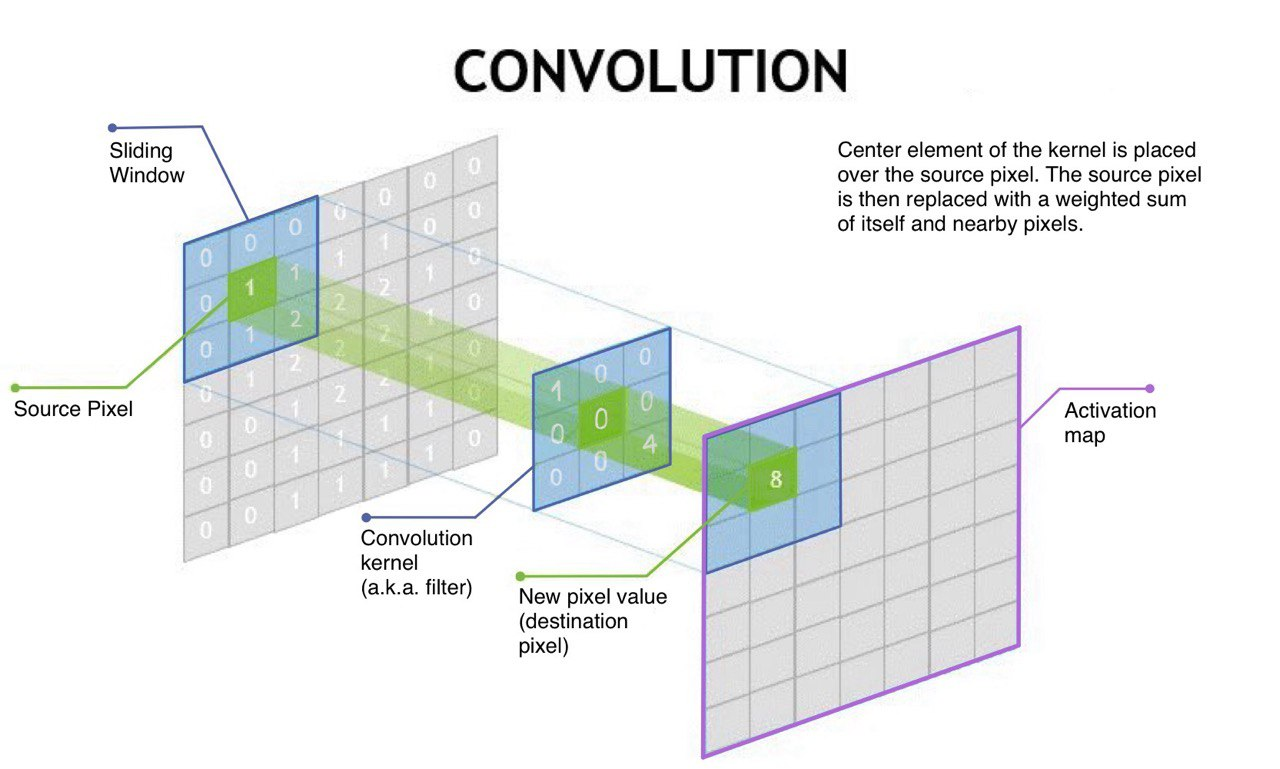
\includegraphics[width=0.95\textwidth]{capitulos/cap_02/imagenes/convolution_operation.jpg}
    \caption
    [
        Esquema gráfico de la aplicación de un filtro convolucional sobre una región de una imagen.
    ]{
        Esquema gráfico de la aplicación de un filtro convolucional de 3×3 sobre una región de una imagen.
        Adaptado de \cite{nvidia2025convolutionoperation}.
    } 
    \label{fig:conv_op}
\end{figure}

Este proceso se repite al desplazar el filtro por toda la imagen mediante una \textbf{ventana deslizante}, 
generando un \textbf{mapa de activación}, que permite destacar líneas, curvas o texturas simples. Este mapa de
activación preserva la información de la localización de las características, si bien estas pueden ser 
detectadas en cualquier parte de la imagen. Esta propiedad se conoce como \textbf{equivarianza}. 

Las \acrshort{CNN} aprovechan la convolución mediante \textbf{capas convolucionales}. Cada capa convolucional está
compuesta por un conjunto de filtros convolucionales, donde cada uno a su vez tiene tantos \textit{kernels} 
como canales de entrada de la imagen haya en la capa (si es la primera capa convolucional, habrá 1 canal en 
imágenes de escala de grises, o 3 en imágenes RGB). El número de filtros en cada capa, su tamaño y la forma
en que se deslizan sobre la entrada%
\footnote{                                                                      
    Definidos mediante los parámetros de \textit{stride} y \textit{padding}, que controlan el desplazamiento       
    del filtro y la cantidad de relleno alrededor de la entrada, respectivamente.
}
se determinan durante el diseño de la red, mientras que los valores de los \textit{kernels} son parámetros 
entrenables.

Cada filtro convolucional realiza la operación convolucional sobre cada canal con el \textit{kernel} que le 
corresponde. Después, se suman los mapas de activación de cada canal (pixel a pixel) añadiendo un sesgo 
(un mismo valor a todos los píxeles%
\footnote{
    Es por ello que no rompe la propiedad de equivarianza.
}),
generando lo que denominamos como \textbf{mapa de características} (ya que idealmente extrae 
características relevantes). Los mapas de características generados con cada uno de los filtros son los nuevos 
canales, que conforman la salida de la capa convolucional. Esta salida puede ser posteriormente procesada por 
otras capas, permitiendo a la red aprender representaciones jerárquicas cada vez más abstractas de los datos 
de entrada: las primeras capas convolucionales detectarán bordes, cambios de color o texturas básicas; a 
medida que avanzamos en las capas de la red, las combinaciones de estas características simples permite 
identificar formas más complejas, como objetos e incluso composiciones.

Sin embargo, hemos pasado por alto algo fundamental: ¿cómo reunimos la información de dos regiones distantes 
de una imagen en un mismo sitio? Una primera aproximación intuitiva nos diría que los filtros convolucionales 
deben ser progresivamente más grandes, para capturar patrones de mayor tamaño y contexto. No obstante, esto
incrementaría considerablemente el número de parámetros y, por tanto, aumentaría el coste computacional y 
el riesgo de sobreajuste del modelo (ya que un modelo con más parámetros puede memorizar mejor los
datos de entrenamiento). Es por esto que, en aquellos problemas en los que no es necesario preservar la 
información de localización de las características, ---como en los que nos enfocamos en este trabajo: 
clasificación y regresión---, y, por tanto, el modelo sea invariante a la ubicación, se emplean técnicas de 
submuestreo (\textit{downsampling}) \cite{murphy2022}, como emplear usar capas de \textit{pooling} o usar \textit{stride} mayor de 1 en los filtros de las capas convolucionales.





\subsubsection{Capas de pooling}

Las \textbf{capas de agrupación (\textit{pooling layers})} tienen como objetivo principal comprimir la 
información de la imagen, reduciendo sus dimensiones (alto y ancho) mientras se preservan los datos más 
relevantes para la tarea. Esta reducción del tamaño espacial de los mapas de características disminuye el 
número de parámetros y operaciones en las fases posteriores, lo que reduce el coste computacional. Además, 
tiene un beneficio adicional: ayuda a prevenir el sobreajuste, ya que al limitar la cantidad de parámetros, 
el modelo evita memorizar ruido o detalles irrelevantes de los datos de entrenamiento, favoreciendo así el 
aprendizaje de patrones generalizables.

Hay diversas operaciones de \textit{pooling}, entre los que destacan:

\begin{itemize}

    \item \textbf{Max pooling}, que calcula el máximo valor de regiones del mapa de características, y lo
    usa para crear un mapa de características reducido (véase la Figura \ref{fig:max_pooling}).

    \item \textbf{Average pooling}, que reemplaza el valor máximo del \textit{max pooling} por el cálculo de
    la media entre los valores de la región. 

\end{itemize}

\begin{figure}[h]
    \centering
    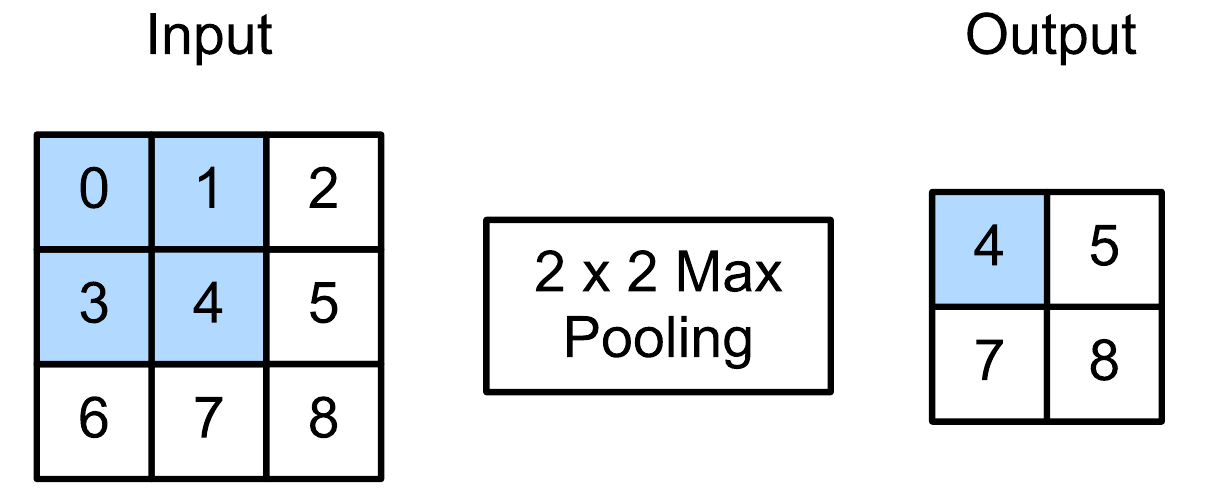
\includegraphics[width=0.7\textwidth]{capitulos/cap_02/imagenes/max_pooling.png}
    \caption[
        Esquema gráfico de aplicación de \textit{max pooling} con un filtro 2×2 y \textit{stride} de 1.
    ]{
        Esquema gráfico de aplicación de \textit{max pooling} con un filtro 2×2 y \textit{stride} de 1.
        Recuperado de la Figura 14.12 de \cite{murphy2022}.
    } 
    \label{fig:max_pooling}
\end{figure}

La región de aplicación del \textit{pooling}, al igual que en la convolución, viene determinada por ciertos 
parámetros, definidos por el diseñador, como el tamaño de filtro (que suele ser de 2×2), el \textit{stride} 
y el \textit{padding}, si bien también existen variantes  adaptativas (\textit{adaptive}), que ajustan
automáticamente su cobertura para producir una salida con dimensiones específicas, independientemente del 
tamaño de la imagen de entrada. Esta funcionalidad es especialmente útil cuando se necesita adaptar los mapas
de características para conectarlos a una capa \textit{fully-connected}. 





\subsubsection{Reducción de dimensionalidad mediante \textit{stride} aumentado}

En una convolución estándar, un filtro se desliza sobre la imagen con un desplazamiento determinado. El \textit{stride} indica cuántos píxeles se mueve el filtro en cada paso:

\begin{itemize}
    \item \textit{Stride} de 1: El filtro se mueve un píxel a la vez. Esto mantiene la mayor parte de la información espacial.
    \item \textit{Stride} de 2: El filtro se mueve dos píxeles a la vez, saltándose algunas posiciones. Esto reduce el tamaño de la salida (\textit{feature map}), lo que se conoce como submuestreo o \textit{downsampling}. Véase la Figura \ref{fig:stride_example}.
\end{itemize}

\begin{figure}[htbp]
    \centering
    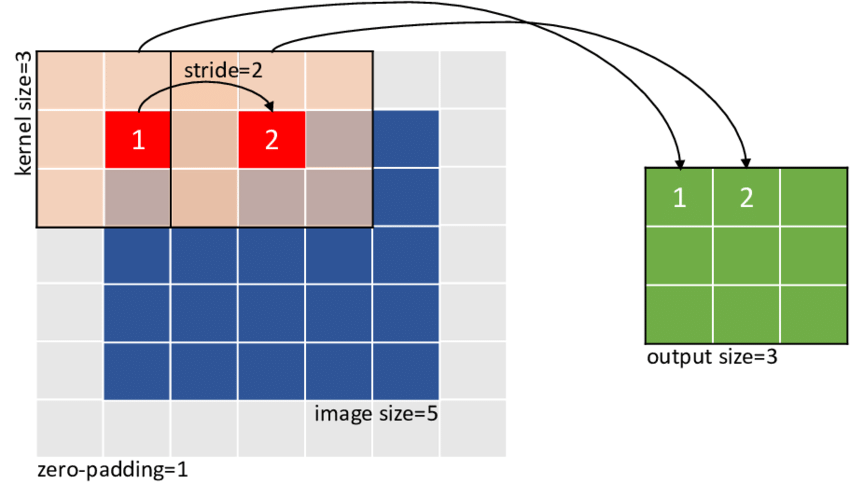
\includegraphics[width=0.7\textwidth]{capitulos/cap_02/imagenes/Example-of-a-square-image-convolution-with-zero-padding-While-training-a-CNN-there-are.png}
    \caption[
        Esquema gráfico de aplicación de un filtro convolucional de 3x3 con \textit{zero-padding} de 1 y \textit{stride} de 2.
    ]{
        Esquema gráfico de aplicación de un filtro convolucional de 3x3 con \textit{zero-padding} de 1 y \textit{stride} de 2.
        Recuperado de la Figura 3 de \cite{kiourt2020deep}.El \textit{zero-padding} consiste en agregar filas y columnas de ceros alrededor de la imagen, de forma que los bordes puedan ser procesados por el filtro sin reducir excesivamente el tamaño del \textit{feature map} resultante. Esto permite que la convolución considere todas las regiones de la imagen, incluyendo los bordes, y facilita la preservación de la información espacial. Con un \textit{stride} de 2, el filtro se desplaza de dos en dos píxeles, realizando simultáneamente la extracción de características y el \textit{subsampling}, lo que genera una reducción controlada del tamaño de salida.
    } 
    \label{fig:stride_example}
\end{figure}


\subsubsection{Capas \textit{Fully-Connected}}

Como hemos visto hasta ahora, en las \acrshort{CNN}, las primeras capas están diseñadas para extraer características espaciales a través de filtros convolucionales y de \textit{pooling}. Sin embargo, una vez que se ha reducido la dimensionalidad y se han obtenido representaciones abstractas de alto nivel, es necesario realizar una predicción (en problemas de clasificación y regresión). Aquí es donde las \textbf{capas completamente conectadas (\textit{fully-connected}, \acrshort{FC})} juegan un papel crucial. Se utilizan en las últimas etapas de la red convolucional para combinar todas las características extraídas y producir una predicción final. Es decir, actúan como el clasificador/regresor%
\footnote{
    Si bien, independientemente de la tarea ---regresión o clasificación---, a esta parte de la red se le 
    denomina clasificador
} 
que toma todas las señales procesadas por las capas anteriores y predice la clase a la que pertenece la imagen o el valor objetivo. 

La arquitectura de esta capa sigue la estructura del \acrshort{MLP}, con neuronas organizadas en una o más capas densas, donde cada neurona está conectada con todas las salidas de la capa anterior. Para que esto sea posible, primero se aplica una operación de \textbf{\textit{flattening}} que transforma el mapa de características multidimensional en un vector unidimensional. A partir de ahí, el procesamiento es equivalente al de una red neuronal tradicional: cada neurona calcula una combinación lineal de sus entradas seguida de una función de activación no lineal.


\subsubsection{Diseño de la CNN para problemas de clasificación y regresión}

Un patrón común de diseño de \acrshort{CNN} para la resolución de problemas de clasificación y regresión consta de dos
componentes principales:

\begin{itemize}

    \item el \textit{backbone} o extractor de características, que alterna capas convolucionales con capas de
    \textit{pooling}, cuya función es extraer representaciones jerárquicas y cada vez más abstractas de los 
    datos de entrada; y

    \item el \textit{classifier}, generalmente implementado mediante una o más capas \acrshort{FC}, 
    toma estas representaciones para realizar la tarea específica de salida, ya sea clasificación o regresión.

\end{itemize}

En la Figura \ref{fig:CNN_complete} se puede observar un ejemplo de arquitectura \acrshort{CNN} completa. 


\begin{figure}[htbp]
    \centering
    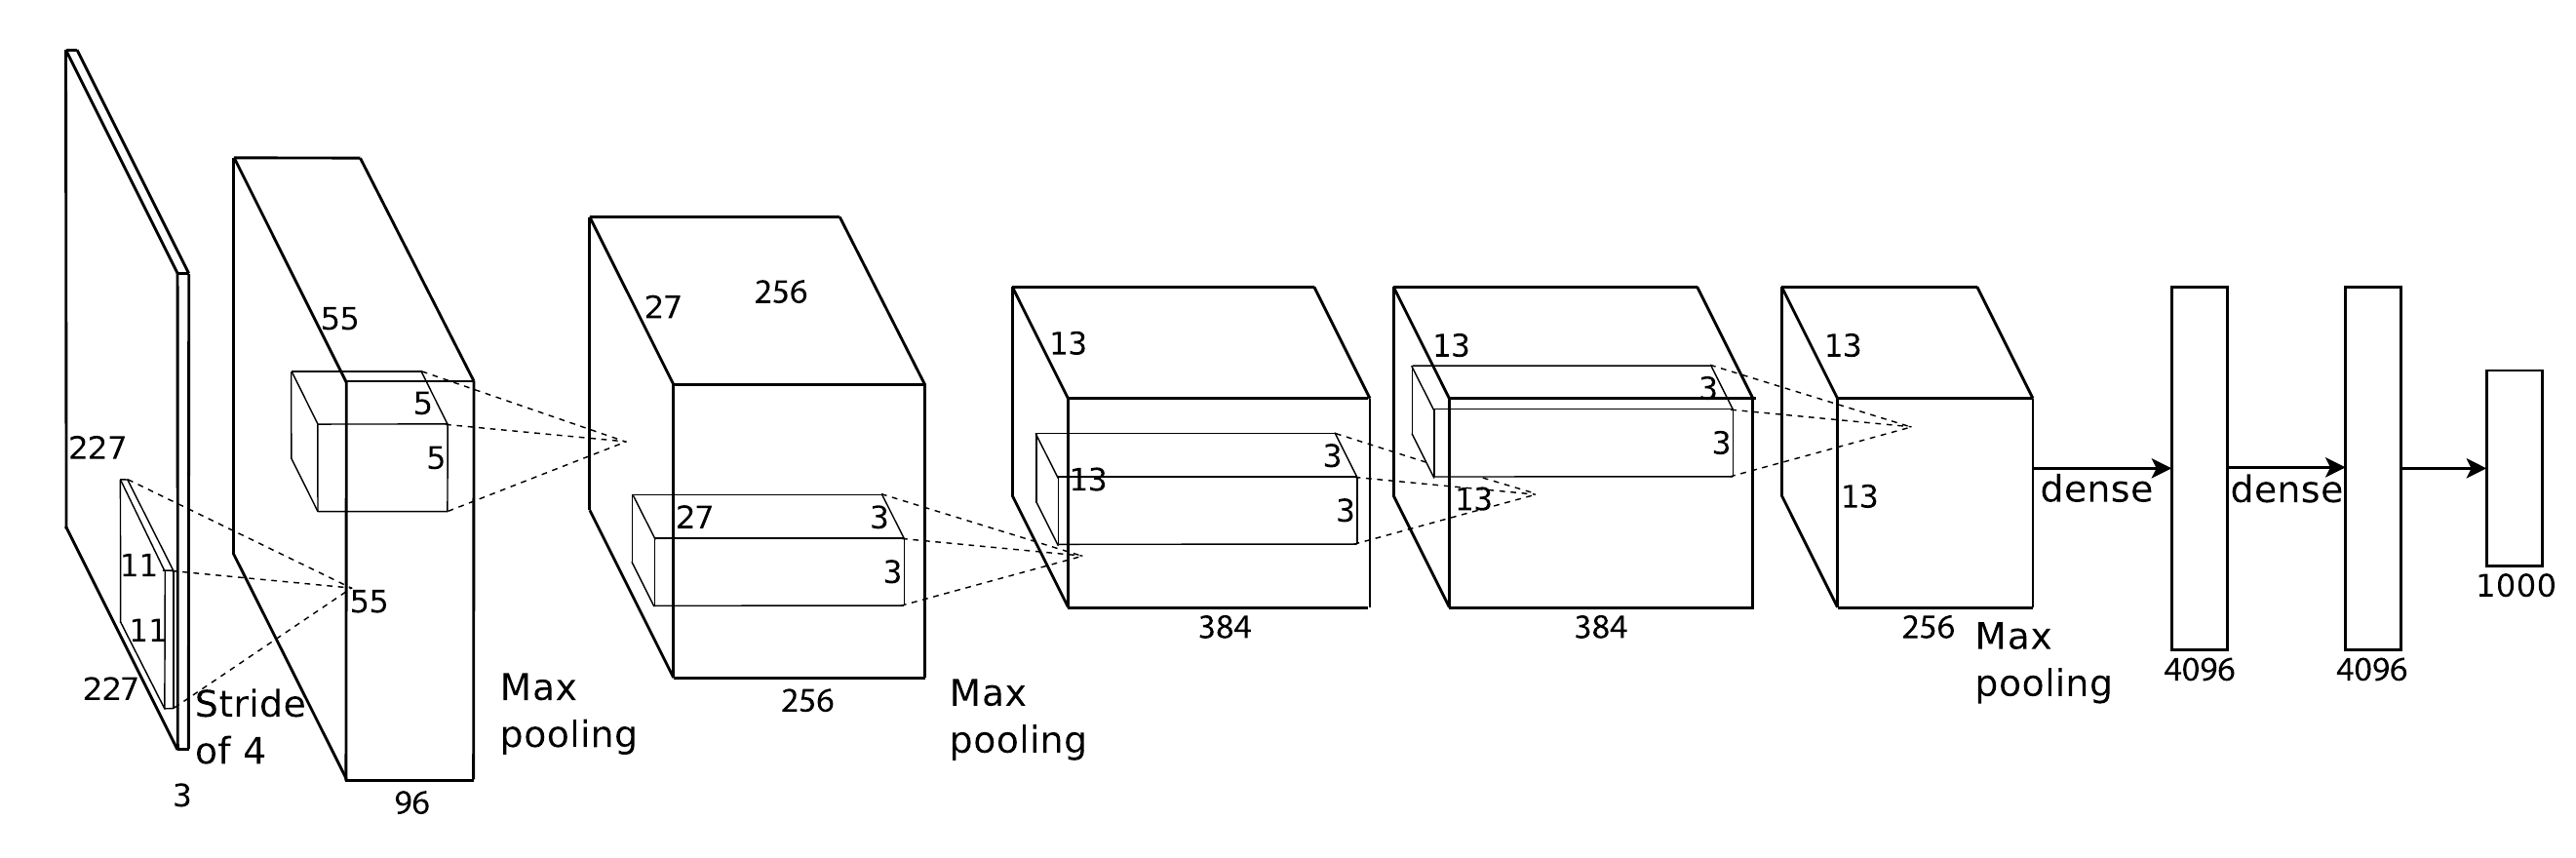
\includegraphics[width=0.95\textwidth]{capitulos/cap_02/imagenes/CNN_complete.png}
    \caption[
       Diagrama de la arquitectura de la red neuronal convolucional ``AlexNet''.
    ]{
        Diagrama de la arquitectura de la red neuronal convolucional ``AlexNet'', diseñada para resolver un problema de clasificación con 1000 clases.
        Recuperado de la Figura 5.39 de \cite{szeliski2010}.
        Esta arquitectura presenta una serie de capas convolucionales con funciones de activación no lineales ReLU y \textit{max pooling}, que formarían el \textit{backbone} y una serie de capas \acrshort{FC} (\textit{classifier}), con una capa final \textit{softmax}, que alimenta una función de pérdida de entropía cruzada multiclase.
    } 
    \label{fig:CNN_complete}
\end{figure}


\subsubsection{Regularización y normalización}

Como en otras arquitecturas de redes neuronales, existen numerosas técnicas de regularización para evitar el sobreajuste. Veamos algunas de las técnicas empleadas en \acrshort{CNN}:

\begin{itemize}

    \item \textbf{\textit{Data augmentation}} \cite{chen2019,zhang2021}: Consiste en añadir o modificar dinámicamente ejemplos a partir de los que se tienen originalmente, de forma que se entrene la red con un conjunto de datos más diverso y robusto, evitando el sobreajuste y mejorando la generalización.
    
    Algunas alteraciones realizadas pueden ser cambios en el nivel de brillo y contraste, rotaciones, traslaciones, escalados o volteos de imágenes, entre otras. No existe configuración óptima, y su configuración depende mucho del problema y las imágenes disponibles.

    Esta técnica sirve especialmente para problemas como clasificación o regresión, donde las clases o valores predichos no suelen variar bajo pequeñas perturbaciones locales. 
    
    \item \textbf{\textit{Dropout}} \cite{srivastava2014}: Técnica que, durante el entrenamiento, ``apaga'' (pone a cero) aleatoriamente un porcentaje de neuronas en cada iteración, evitando así que la red dependa demasiado de determinadas unidades individuales (véase la Figura \ref{fig:net_with_dropout}). En \acrshort{CNN} suele aplicarse a capas \acrshort{FC}, aunque existen variantes como \textit{Spatial Dropout} \cite{tompson2015} que elimina canales completos en capas convolucionales, forzando una distribución más robusta de características.

    \begin{figure}[htbp]
        \centering

        \begin{subfigure}[b]{0.45\textwidth}
            \centering
            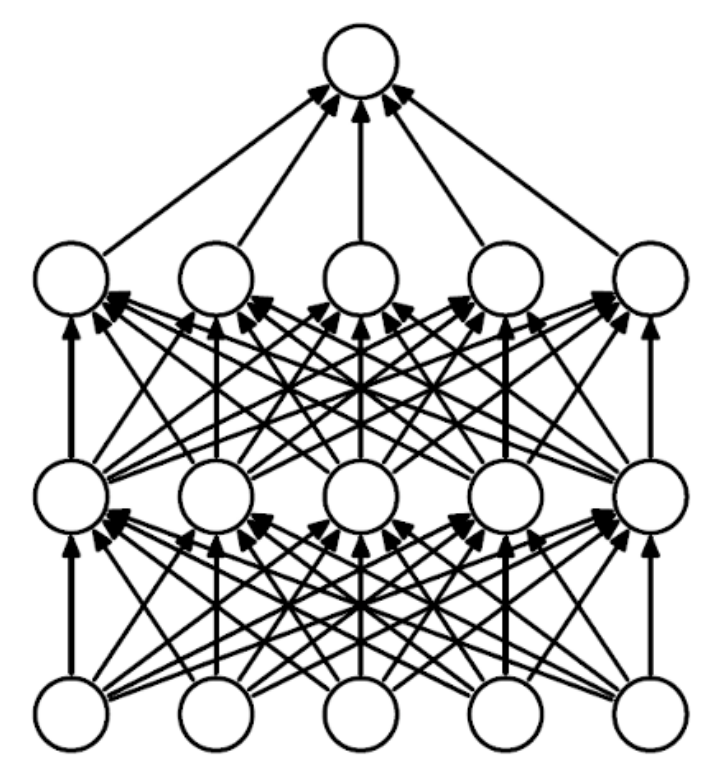
\includegraphics[width=\textwidth]{capitulos/cap_02/imagenes/net_without_dropout.png}
            \caption{Dropout desactivado}
            \label{fig:net_deactivate_dropout}
        \end{subfigure}
        \hfill
        \begin{subfigure}[b]{0.45\textwidth}
            \centering
            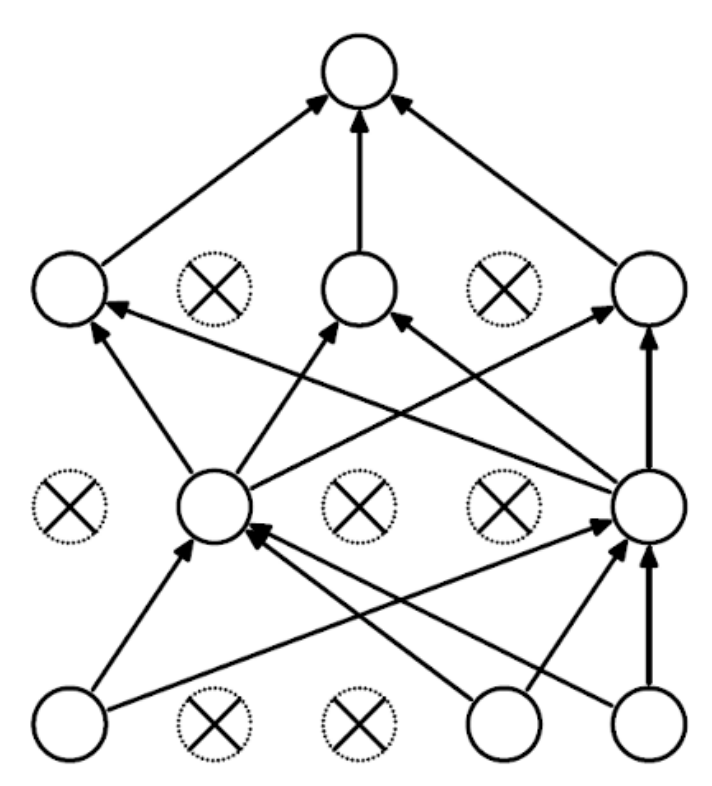
\includegraphics[width=\textwidth]{capitulos/cap_02/imagenes/net_with_dropout.png}
            \caption{Dropout activado ($p=0.5$)}
            \label{fig:net_activate_dropout}
        \end{subfigure}

        \caption[
            Esquema gráfico del funcionamiento de neuronas con \textit{dropout}.
        ]{
            Esquema gráfico del funcionamiento de neuronas con \textit{dropout}.
            Recuperado de la Figura 5.29 de \cite{szeliski2010}.
            Cuando se evalúa el modelo, todas las unidades funcionan correctamente (\ref{sub@fig:net_deactivate_dropout}). Durante el entrenamiento, algunas son ``apagadas'' (\ref{sub@fig:net_activate_dropout}). 
        }
        \label{fig:net_with_dropout}
    \end{figure}
    
    \item \textbf{\textit{Batch normalization}} \cite{ioffe2015}: Esta se introduce como una capa nueva a 
    añadir en el diseño de las redes, con nuevos parámetros entrenables: \textit{scale} y \textit{shift}. 
    Normaliza los valores de cada canal (media cero y desviación 1), y los reescala y desplaza en base a los
    valores de \textit{scale} y \textit{shift}. 
    Esto suaviza significativamente el espacio de valores de optimización \cite{santurkar2019} y reduce la 
    sensibilidad a la tasa de aprendizaje \cite{arora2018}, permitiendo establecer valores más altos.
    En CNNs se aplica típicamente después de las capas convolucionales y antes de la función de activación
    
\end{itemize}


% \subsubsection{Conexiones residuales}

% Uno de los principales problemas que no permite aumentar mucho la profundidasd de las redes convolucionales 
% es el desvanecimiento de gradiente (\textit{vanishing gradient problem}), que consiste en la disminución 
% exponencial de los gradientes durante el proceso de \textit{backpropagation} a medida que se retrocede hacia 
% las capas iniciales de la red. Algunas de las soluciones a este problema han sido: utilizar funciones de 
% activación ReLU, ya que evita gradientes pequeños para valores positivos; inicializar adecuadamente los pesos
% de la red; o \textit{batch normalization}, que estabiliza la distribución de las activaciones. Sin embargo,
% las conexiones residuales han sido la contribución más significativa para resolver este problema.

% Las \textbf{redes residuales (\textit{residual nets}, ResNet)} 

% \todo{Por completar (AGOSTO)}

%https://www.jeremyjordan.me/nn-learning-rate/



% ------------------------------------------------------------------------------------------------------------

\subsection{Transfer Learning}

El \textbf{aprendizaje por transferencia (\textit{transfer learning})} es una técnica que consiste en 
aprovechar el conocimiento aprendido por un modelo entrenado en una tarea como punto de partida para
mejorar el rendimiento y acelerar el entrenamiento en una nueva tarea relacionada \cite{rusell2021}.
En redes neuronales, el aprendizaje consiste en ajustar pesos, y en el caso del \textit{transfer learning}, 
estos pesos se inicializan con valores previamente optimizados para una tarea fuente, en lugar de comenzar con valores aleatorios (véase la Figura \ref{fig:fine-tuning}).

Se conoce como \textbf{fine-tuning} a la técnica de inicialización de los pesos de aquellas partes del modelo (como capas convolucionales) con los pesos previamente aprendidos, y que continúa el entrenamiento con los datos específicos de la nueva tarea. En este contexto, se denomina \textit{head} a las capas finales del modelo que se sustituyen para adaptarse a la nueva tarea. Por ejemplo, en \cite{venema2022} se utilizan dos modelos de \acrshort{CNN} preentrenados en clasificación con ImageNet (que contiene imágenes de 1000 clases): VGG16 y ResNet50. Estos modelos se ajustan (\textit{fine-tuning}) para estimar el sexo de una persona a partir de radiografías de húmero. Aunque ambas tareas parecen muy diferentes, las primeras capas de la red, especializadas en detectar características generales como bordes y texturas, pueden ser útiles en los dos casos, lo que permite una transferencia efectiva del conocimiento. El \textit{fine-tuning} puede aplicarse de forma gradual: primero se entrena solo el \textit{head} (manteniendo el resto del modelo congelado) y luego, si es necesario, se afinan también algunas capas  preentrenadas para mejorar el rendimiento en la tarea específica.

\begin{figure}[h]
    \centering
    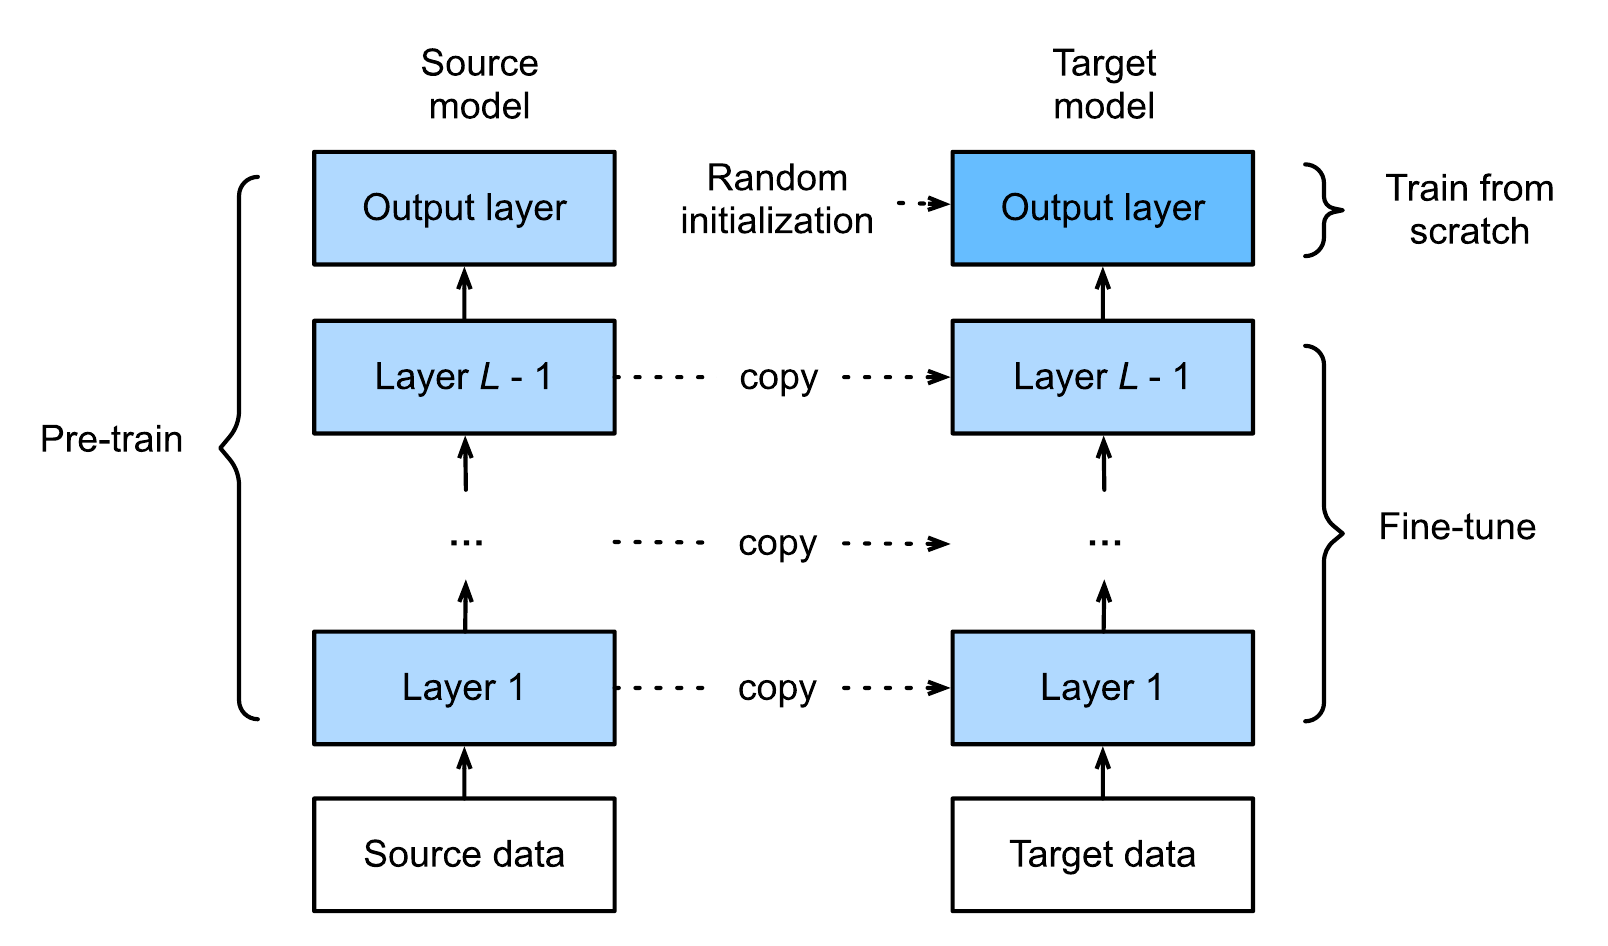
\includegraphics[width=0.95\textwidth]{capitulos/cap_02/imagenes/fine-tunning.png}
    \caption[
        Diagrama del proceso de \textit{fine-tuning} de un modelo de red neuronal en una nueva tarea.
    ]{
        Diagrama del proceso de \textit{fine-tuning} de un modelo de red neuronal en una nueva tarea. 
        Recuperado de la Figura 19.2 de \cite{murphy2022}.
        La capa final de salida es entrenada desde cero para la nueva tarea. El resto de capas son 
        inicializadas con los pesos previos. 
    } 
    \label{fig:fine-tuning}
\end{figure}

% ------------------------------------------------------------------------------------------------------------
% INCERTIDUMBRE ----------------------------------------------------------------------------------------------
% ------------------------------------------------------------------------------------------------------------

\section{Incertidumbre}

La metrología%%%
\footnote{
    Ciencia de las mediciones y sus aplicaciones \cite{jcgm200:2012}.
},
y la estadística comparten un papel fundamental en el análisis del error y la incertidumbre en campos como 
el \acrshort{ML}. Mientras la metrología establece los fundamentos conceptuales de error e incertidumbre, la estadística proporciona métodos para cuantificar, modelar y reducir estos factores durante el desarrollo y validación de modelos.

El Comité Conjunto de Guías en Metrología (\textit{Joint Committe for Guides in Metrology})%%
\footnote{
    Este Comité está formado por numerosas organizaciones internacionales de metrología y normalización: 
    BIPM, IEC, IFCC, ISO, IUPAC, IUPAP, OIML e ILAC. Su objetivo principal es mantener y promover las 
    guías internacionales clave en metrología, como la Guía para la Expresión de la Incertidumbre en la 
    Medición (\textit{Guide to the Expression of Uncertainty in Measurement}) \cite{jcgm100:2008} y el 
    Vocabulario Internacional de Metrología (\textit{Vocabulaire international de métrologie}) 
    \cite{jcgm200:2012}.
} 
define el \textbf{error} como una ``medición imperfecta'' de la magnitud observada, que puede estar causada por efectos aleatorios (componente aleatoria del error) y por efectos sistemáticos (componente sistemática del error, más conocida como \textbf{sesgo}). Por otro lado, define a la \textbf{incertidumbre} como ``parámetro, asociado con el resultado de una medición, que caracteriza la dispersión de los valores que podrían atribuirse razonablemente al \textbf{mensurado}, que es como se denomina a la magnitud a ser medida. [...] El parámetro puede ser, por ejemplo, una desviación estándar, o la amplitud de un intervalo con un nivel de confianza establecido'' \cite{jcgm100:2008}.

Partiendo de estas definiciones generales, veamos las diferencias entre los dos enfoques principales en la evaluación de mediciones: el enfoque basado en el error y el enfoque basado en la incertidumbre.

El \textbf{enfoque basado en el error} o enfoque tradicional parte de la premisa de que existe un valor verdadero. En consecuencia, el propósito de la medición es aproximarse lo máximo posible a dicho valor, minimizando las distintas componentes del error \cite{jcgm100:2008}:

\begin{itemize}

    \item para el error aleatorio, esto se logra aumentando el número de observaciones, ya que su distribución tiende a una media igual a cero; y

    \item para el error sistemático, es necesario identificarlo y cuantificar su magnitud, lo que permite aplicar factores de corrección que compensen su efecto.

\end{itemize}

% Se asume que el resultado de la medición ha sido corregido por todos los efectos sistemáticos identificados
% como significativos, de modo que la esperanza matemática de esta componente sea igual a cero.

Sin embargo, en la práctica no existen reglas claras para distinguir las componentes del error ni cómo estas se combinan en el error total. En general, solo es posible estimar un límite superior del valor absoluto del error total estimado, al que se denomina de forma inapropiada ``incertidumbre''. 

Frente al enfoque anterior, se presenta el \textbf{enfoque basado en la incertidumbre} \cite{jcgm100:2008}, cuyo propósito no es hallar el mejor valor posible, sino establecer un intervalo de valores razonables para el mensurando, el cual puede refinarse con información adicional. Así, la medición misma se convierte en una herramienta para determinar el error potencial del instrumento ---o modelo en \acrshort{ML}---. 

% ------------------------------------------------------------------------------------------------------------

\subsection{Incertidumbre en \textit{machine learning}}

Las fuentes de incertidumbre pueden ser muy variadas, y su identificación requiere en muchos casos de 
conocimiento específico del problema. No obstante, en términos prácticos, suelen considerarse dos tipos de 
incertidumbre en las predicciones realizadas en \acrshort{ML} \cite{hullermeier2021, nemani2023}:

\begin{itemize}
    
    \item La \textbf{incertidumbre aleatoria o estocástica} procede de la variabilidad aleatoria de un 
    fenómeno. Es irreducible por naturaleza, aunque se disponga de más datos. Un ejemplo típico es el resultado de lanzar una moneda al aire. Incluso el mejor modelo solo será capaz de dar probabilidades para las dos posibles salidas, sin una respuesta definitiva. En el contexto de la estimación de la edad forense, esta incertidumbre se manifiesta en las diferentes edades biológicas que pueden obtenerse para individuos de la misma edad cronológica. Se sabe que existe una correlación entre edad biológica y la cronológica, pero esta no es perfecta, debido a que existe variabilidad inherente al problema.

    % \begin{itemize}
    %     \item las entradas. Por ejemplo, 
        
    %     \item las salidas. Por ejemplo, el resultado de lanzar una moneda al aire; incluso el mejor modelo 
    %     solo será capaz de dar probabilidades para las dos posibles salidas, sin una respuesta definitiva.
        
    %     \item la dependencia entre las anteriores. Por ejemplo, estimar la edad cronológica de un esqueleto  
    %     un esqueleto de determina edad biológica
    
    % \end{itemize}


    \item La \textbf{incertidumbre epistémica} es la causada por falta de conocimiento o precisión del modelo.Se relaciona con aspectos como la escasez de datos, la calidad de la información disponible, las limitaciones teóricas y prácticas del modelo escogido, etc. A diferencia de la incertidumbre aleatoria, esta sí es reducible por naturaleza; puede reducirse con más datos, mejores modelos o mayor comprensión del problema. 
    
\end{itemize}

A estos, se les puede añadir un tercer tipo: el \textbf{\textit{drift}} \cite{gama2012, nemani2023}, que procede de cambios en la distribución de los datos a lo largo del tiempo, ya sea en la distribución de las variables de entrada, en la distribución de las variables de salida, o en la relación entre las dos previas. Por ejemplo, una imagen de entrada a un modelo de clasificación que no corresponde a ninguna clase con la que se haya entrenado anteriormente; un cambio en la población objetivo de una aplicación médica ---p.ej., debido a un cambio demográfico o a la aparición de una nueva enfermedad---; o la toma de imágenes médicas con una máquina distinta a la que se empleó para obtener las imágenes con las que se ha entrenado el modelo.

% ------------------------------------------------------------------------------------------------------------

\subsection{Cuantificación de la incertidumbre en \textit{machine learning}} 

El desarrollo de las técnicas modernas de \acrshort{ML} se asocia con un enfoque basado en el error, centrándose en la minimización y cuantificación del error en predicción. Este enfoque ha permitido que el aprendizaje automático despliegue un gran potencial en multitud de aplicaciones. Sin embargo, cuando se trata de aplicaciones críticas ---como la medicina, los sistemas financieros o el control de infraestructuras--- surge una necesidad esencial: no solo importa cuán precisa es una predicción, sino también cuán confiable es \cite{begoli2019}. En respuesta a esta necesidad, durante la última década se ha producido un creciente interés y desarrollo de técnicas orientadas a la explicabilidad e interpretabilidad de la \acrshort{IA} \cite{angelov2021, ali2023, miller2019, loh2022} y la cuantificación de la incertidumbre \cite{abdar2021, psaros2023, nemani2023}.

Mientras la explicabilidad de la \acrshort{IA} busca entender las razones detrás de cada predicción centrándose en el estudio del modelo y arquitectura concretos \cite{salvi2025}, la \textbf{cuantificación de la incertidumbre (\textit{uncertainty quantification}, \acrshort{UQ})} evalúa el grado de confianza en las predicciones realizadas y se centra en caracterizar las fuentes de variabilidad y posible error en los datos, el modelo y el entorno de aplicación \cite{nemani2023}.

Existe una gran variedad de técnicas de \acrshort{UQ}. Estas técnicas pueden clasificarse de distintas formas: 

\begin{itemize}

    \item Algunas son \textit{model-agnostic}, es decir, pueden aplicarse a cualquier tipo de modelo sin 
    requerir acceso a su estructura interna; otras son \textit{model-specific}, diseñadas para aprovechar 
    características particulares del modelo subyacente. 

    \item Algunas técnicas suponen que los datos siguen ciertas distribuciones estadísticas explícitas, 
    mientras que otras operan sin realizar tales suposiciones.

    \item También existen técnicas que asumen intercambiabilidad entre observaciones, frente a aquellos que 
    no lo hacen y requieren estructuras de dependencia más complejas. 

\end{itemize} 


Algunas técnicas específicas de \acrshort{UQ} en modelos \acrshort{ML} se dividen en cuatro grupos:

\begin{itemize}

    \item \textbf{Procesos de regresión gausiana (\textit{gaussian process regression})}: 
    Modelos no paramétricos que proporcionan una distribución completa sobre funciones posibles, permitiendo obtener predicciones con intervalos de confianza naturales. Son especialmente útiles en problemas de regresión con pocos datos y cuando la estimación de incertidumbre es crítica \cite{rasmussen2003}.

    \item \textbf{Redes neuronales bayesianas}: \textit{Markov Chain Monte Carlo} \cite{neal2012}, \textit{Variational Inference} \cite{blundell2015} y \textit{Monte Carlo Dropout} \cite{gal2016} incorporan incertidumbre de manera explícita en los parámetros del modelo o en la estructura de la red, generando distribuciones sobre las predicciones en lugar de valores puntuales.

    \item \textbf{Técnicas \textit{ensemble}}: Agrupan múltiples modelos independientes o variantes del mismo modelo para mejorar la robustez de las predicciones. La variabilidad entre los miembros del \textit{ensemble} se utiliza como medida de incertidumbre. Ejemplos incluyen \textit{bagging}, \textit{boosting} y \textit{deep ensembles} \cite{opitz1999}.

    \item \textbf{Métodos deterministas}: Aproximaciones que estiman la incertidumbre sin recurrir a técnicas probabilísticas, generalmente mediante reformulaciones del modelo que generan límites superiores e inferiores sobre las predicciones, como los métodos basados en \textit{predicción conformal} \cite{papadopoulos2002, sadinle2019, angelopoulos2021}.
    
\end{itemize}

En este trabajo exploraremos la predicción el método determinista de predicción conformal, de los métodos más flexibles que hay: mayormente \textit{model-agnostic} y aplicable sobre cualquier distribución de datos, si bien sí asume intercambiabilidad entre observaciones. Esta es una técnica fácil de implementar y proporciona intervalos de predicción válidos para un nivel de confianza, permitiendo cuantificar la incertidumbre de manera robusta con conjuntos de datos limitados. 
 
% \todo{Pablo: De hecho, aquí repites cosas... Tal y como dices, se ve que está por completar... Aún así, como consejo para todo lo que falta por completar: no te rayes ni líes mucho. Ya llevas 131 páginas y, bajo ningún concepto, queremos superar por mucho este valor (150 páginas podría estar bien, pero mucho más de eso... me parecería excesivo). Da pinceladas que demuestren que entiendes de lo que hablas, pero sin entrar en demasiado detalle. Si alguien quiere saber más: que se lea las referencias que incluyas y/o que te pregunte durante la defensa.}


% ¿Qué es la cuantificación de incertidumbre?

% Es un proceso añadido sobre el actual proceso de entrenamiento de un modelo, ya sea ..., 
% que genera un intervalo o distribución 




% La UQ puede abordarse desde dos perspectivas diferentes: 

% \begin{itemize}

%     \item sobre datos ya observados (como los de entrenamiento o validación), donde el objetivo es evaluar si 
%     el modelo representa adecuadamente la variabilidad de los datos, detectar sobreajuste o validar la 
%     calibración de las predicciones; o
    
%     \item sobre nuevos datos (no vistos), donde el objetivo es estimar la confianza del modelo en situaciones 
%     reales de predicción, donde no se conoce el valor verdadero.

% \end{itemize}

% Algunos métodos de cuantificación de la incertidumbre

% % Hablar sobre métodos de UQ en datos ya observados

% Nos centraremos en el estudio de la cuantificación de la incertidumbre sobre datos nuevos, pues es en este 
% contexto donde resulta más relevante para aplicaciones prácticas, como las de estimación del PB. 
% Esta provee información clave para la toma de decisiones tanto del valor predicho como de la certeza asociada
% a la predicción. 
% \todo{
%     ¿Es posible hablar de métodos de cuantificación de incertidumbre sobre datos nuevos sin mencionar los
%     métodos sobre datos previos? En clasificación, la calibración del modelo es importante para la 
%     cuantificación de incertidumbre. De hecho, es recomendable realizarla previamente a la aplicación de 
%     conformal prediction.
% }

% En problemas de regresión, es deseable que los modelos no solo proporcionen una 
% predicción puntual, sino también un intervalo que indique el grado de incertidumbre asociado a cada 
% predicción, conocido como \textbf{intervalo de predicción (\textit{prediction interval})},
% el cual puede derivarse de métodos de UQ como %%%%%%AÑADIRR MÁS \textit{bootstrapping} o predicción conformal

% Además, nos centraremos en aquellos métodos que no requieran asumir distribuciones específicas en los datos
% ni dependan fuertemente de supuestos paramétricos, ya que en muchos problemas reales (como la 
% estimación del perfil biológico) los datos pueden presentar heterocedasticidad, asimetría o 
% comportamientos complejos que dificultan su modelización con enfoques clásicos.





% \subsubsection{Cuantificación de la incertidumbre en problemas de regresión}

% Existe multitud de maneras de cuantificar la incertidumbre en problemas de regresión.

% % Comenzar hablando sobre los intervalos de predicción

% % Reestructurar

% Una primera aproximación es la \textbf{regresión cuantílica (\textit{quantile regression})}, que añade dos 
% nuevas salidas en el modelo de regresión, que serán los límites inferior y superior de un intervalo de 
% predicción, correspondientes a cuantiles específicos (por ejemplo, los percentiles 10 y 90)
% \footnote{
%     El entrenamiento del modelo para estas dos salidas se realiza con la función de pérdida \textit{pinball},
%     \cite{steinwart2011} que combina los errores de predicción para múltiples cuantiles, penalizando
%     asimétricamente las desviaciones según el cuantil objetivo.
% }. 
% Esto permite estimar no solo la tendencia central (como en la regresión tradicional), sino también la 
% incertidumbre de las predicciones (véase la Figura \ref{fig:quantile_regression}).

% \begin{figure}[htbp]
%     \centering
%     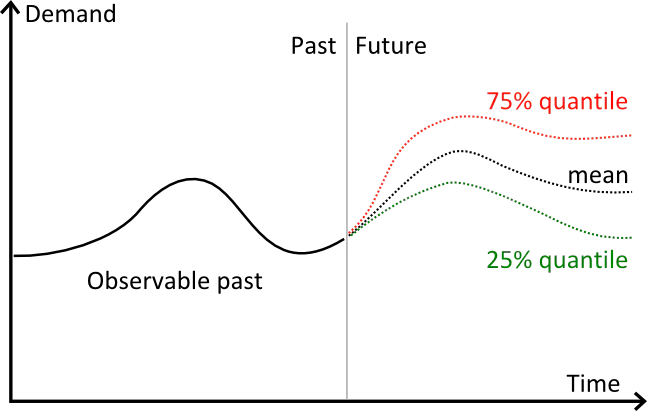
\includegraphics[width=0.8\textwidth]{capitulos/cap_02/imagenes/quantile_regression.png}
%     \caption[
%         Gráfico que ilustra las 3 predicciones que arroja un modelo de regresión cuantílica. Recuperado de 
%         \cite{vermorel2012}.
%     ]{
%         Gráfico que ilustra las 3 predicciones que arroja un modelo de regresión cuantílica. Recuperado de 
%         \cite{vermorel2012}. Se observa los límites superior e inferior los percentiles 75 y 25, 
%         respectivamente. 
%     }
%     \label{fig:quantile_regression}
% \end{figure}

% Sin embargo, este método presenta varios problemas:

% \begin{itemize}

%     \item Sensibilidad a datos escasos o ruidosos: La estimación puede ser muy sensible a 
%     \textit{outliers}
%     \footnote{
%         Los valores atípicos o \textit{outliers} son instancias que se desvían significativamente del resto
%         de instancias del conjunto de datos. Un \textit{outlier} podría indicar un comportamiento anormal
%         del sistema (variabilidad natural del fenómeno observado, eventos excepcionales que refleja 
%         comportamientos reales pero poco frecuentes, ...) o un error de recolección y registro de los datos 
%         \cite{alpaydin2010}.   
%     } 
%     y a regiones con pocas observaciones, llevando a intervalos poco fiables. De hecho, se puede dar el 
%     fenómeno indeseable de que cuantiles mayores tengan valores predichos más bajos que cuantiles menores 
%     ---conocido como cruzamiento de cuantiles \cite{koenker2005}---.
    
%     \item Falta de cobertura probabilística garantizada: No existe ningún tipo de garantía estadística que 
%     asegure que el cuantil estimado cubra la proporción deseada de observaciones en muestras futuras. 
    
%     \item No captura la incertidumbre epistémica: Solo captura la incertidumbre aleatoria \cite{abdar2021},
%     dado que modela cómo los valores de salida varían dado un conjunto de entradas. No captura automáticamente 
%     incertidumbre epistémica, a menos que se combine con otros enfoques, como métodos bayesianos 
%     \cite{tokdar2012}.

%     \item Muestran gran incertidumbre en cuantiles extremos (cerca de cero o uno) \cite{feldman2023} y, por 
%     tanto, los intervalos de predicción obtenidos son extremedamente grandes, lo que logra una gran cobertura
%     pero poca utilidad práctica. 
    
% \end{itemize}





% ------------------------------------------------------------------------------------------------------------
% CONFORMAL PREDICTION ---------------------------------------------------------------------------------------
% ------------------------------------------------------------------------------------------------------------

\section{Predicción conformal}

La \textbf{predicción conformal (\textit{conformal prediction}, \acrshort{CP})} \cite{vovk2005, angelopoulos2021} es un marco teórico para la \acrshort{UQ} en modelos de \acrshort{ML}, que proporciona intervalos o conjuntos de predicción con garantías estadísticas de cobertura, esto es, para una entrada dada $x$, el marco de \acrshort{CP} genera un conjunto de posibles salidas $\hat{C}(x) \subseteq Y$ que garantiza, con una probabilidad predefinida $1-\alpha$, que la verdadera etiqueta o valor $y$ esté contenida en $\hat{C}(x)$ (véanse los ejemplos de la Figura 
\ref{fig:educational_visual}).

\begin{figure}[h]
    \centering
    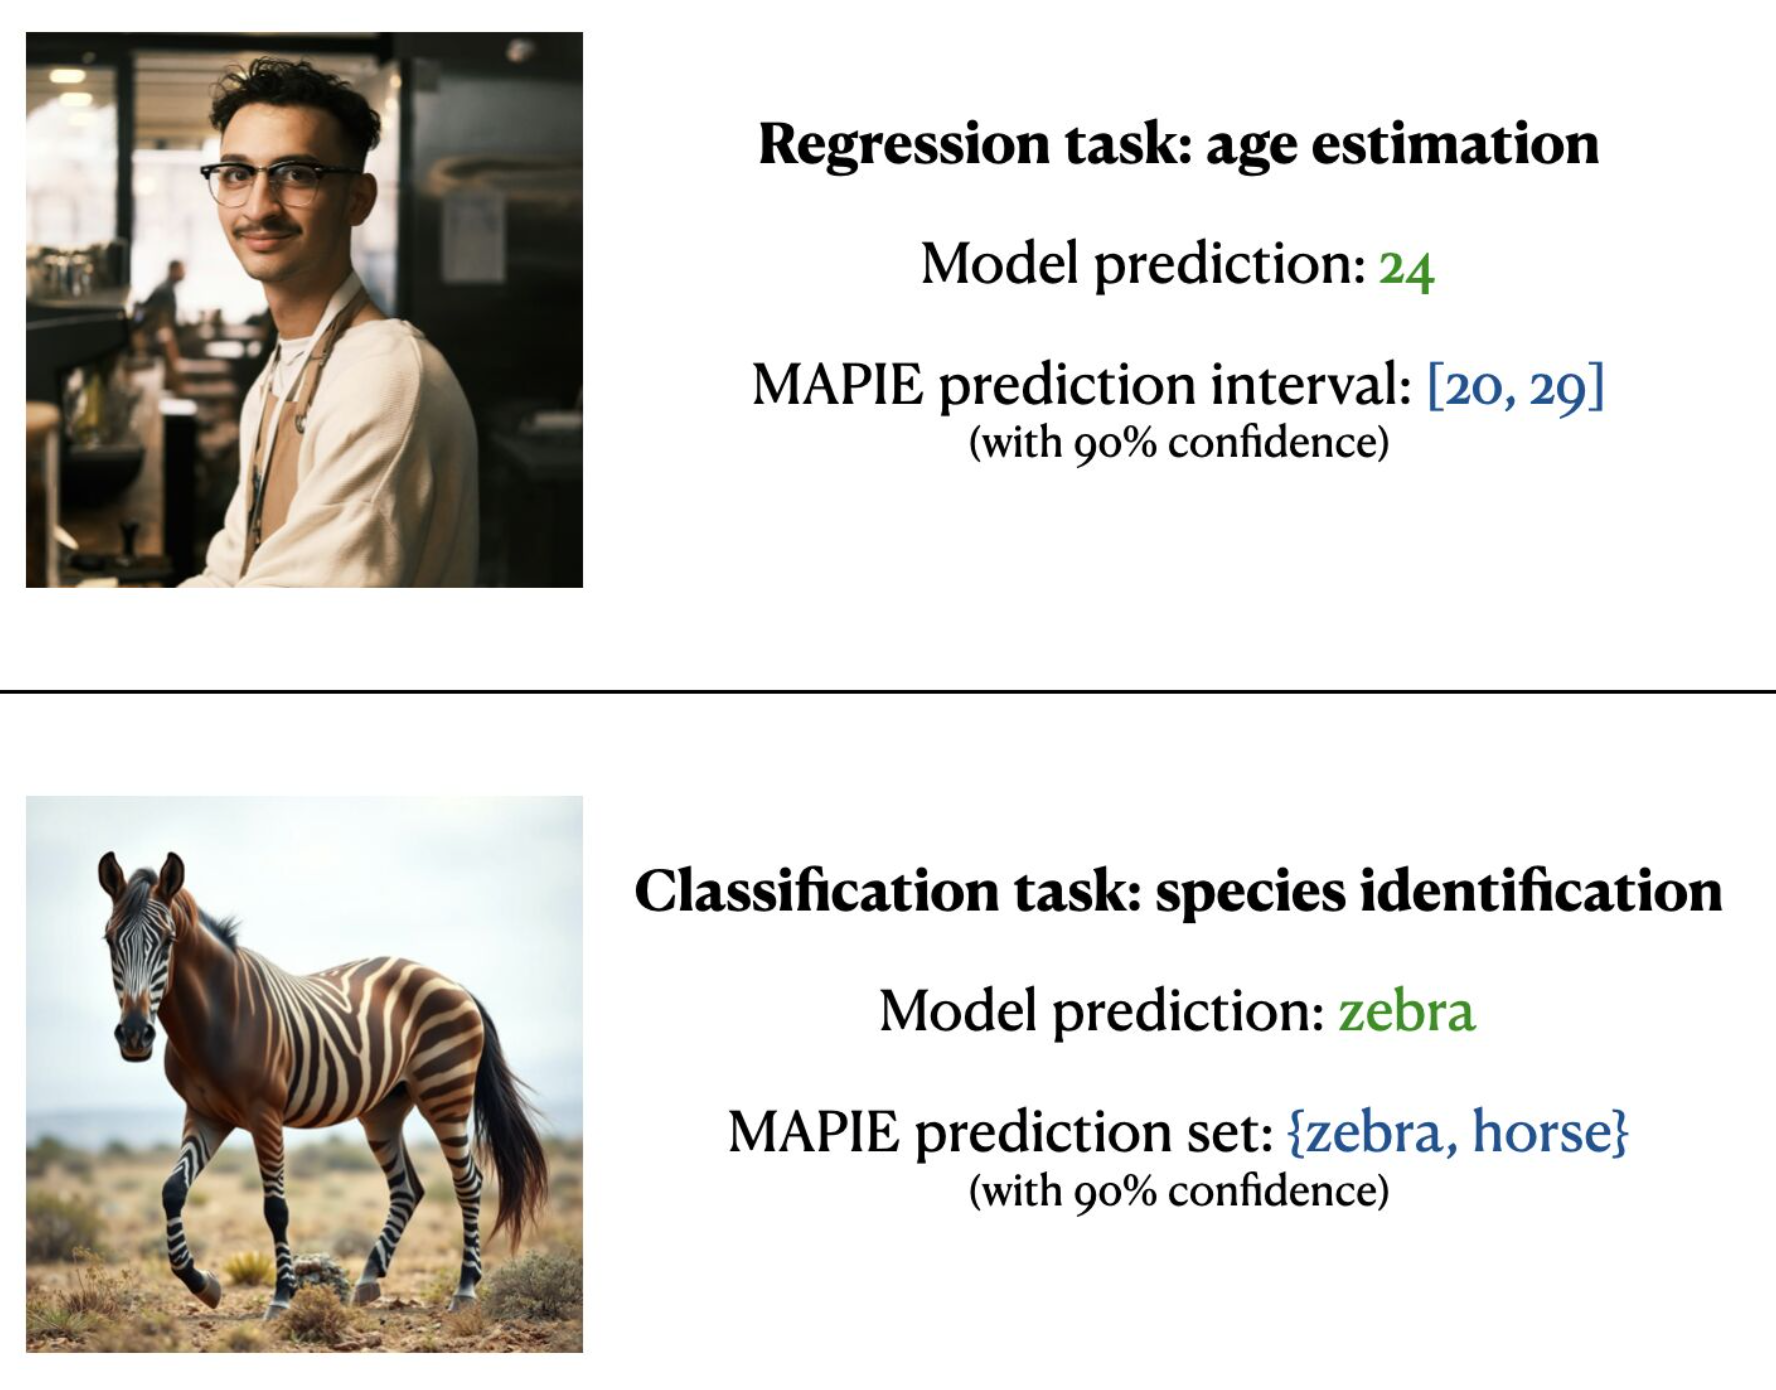
\includegraphics[width=\textwidth]{capitulos/cap_02/imagenes/educational_visual.png}
    \caption[
        Ejemplo de predicción conformal en problemas de regresión y clasificación.
    ]{
        Ejemplo de predicción conformal en problemas de regresión (arriba) y clasificación (abajo).
        Recuperado de \cite{mapie-docs2023}. MAPIE es una biblioteca de Python para la cuantificación
        de incertidumbre, principalmente con técnicas de \acrshort{CP}. 
    } 
    \label{fig:educational_visual}
\end{figure}


Para construir los conjuntos de predicción conformal, se requiere dividir el conjunto de datos disponible en al menos dos partes: un conjunto de entrenamiento, usado para ajustar el modelo base, y un \textbf{conjunto de calibración}, usado para calibrar la predicción conformal, tal y como veremos en los siguiente apartados.Con esto también se busca reducir la variabilidad de las predicciones puntuales, que pueden ser sensibles a pequeños cambios en los datos de entrada, como el ejemplo de la Figura \ref{fig:adversarial_example}. Estas garantías son válidas bajo el supuesto mínimo de intercambiabilidad de los datos, sin requerir hipótesis sobre la distribución subyacente de los mismos. La intercambiabilidad de los datos se refiere a que el orden de las observaciones no aporta información adicional, es decir, la distribución conjunta es invariante ante cualquier permutación de los índices. 

\begin{figure}[htbp]
    \centering
    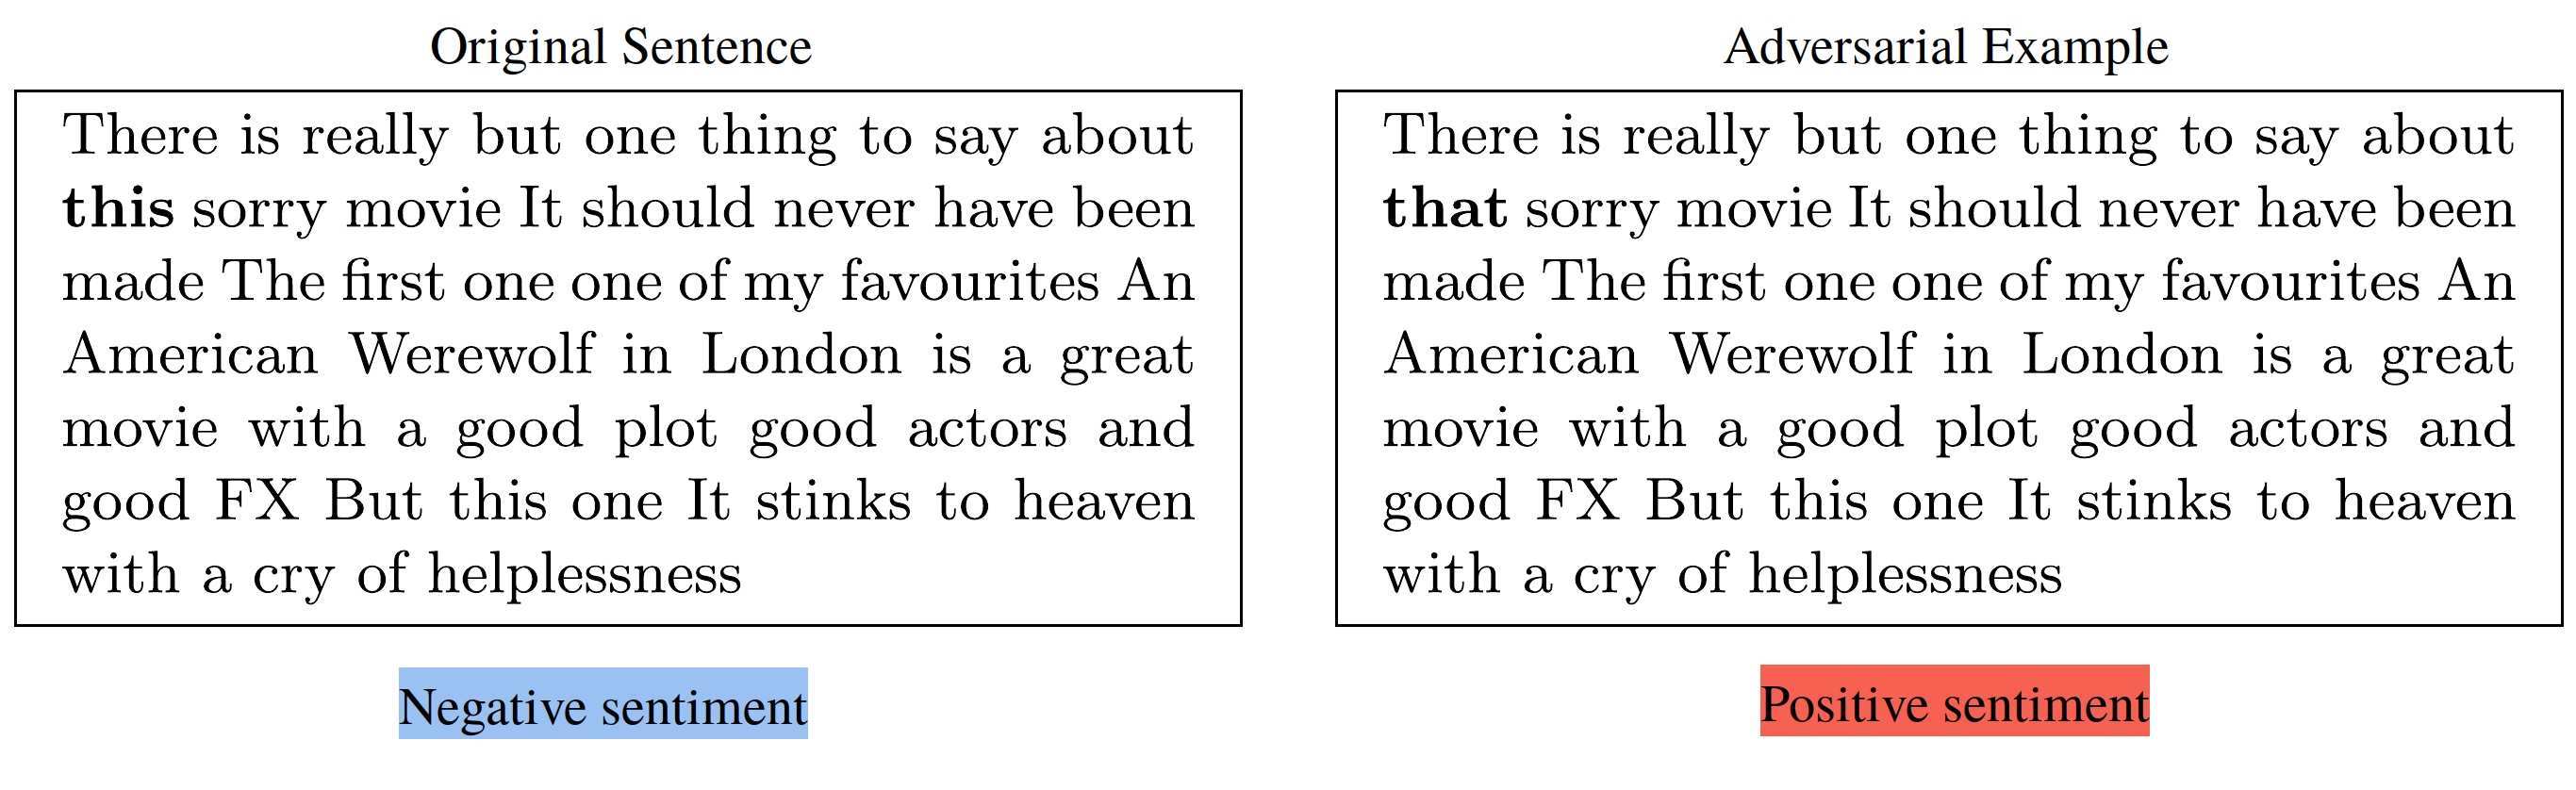
\includegraphics[width=\textwidth]{capitulos/cap_02/imagenes/adversarial_example.png}
    \caption[
        Ejemplo adversario mal clasificado por un modelo de \textit{machine learning} entrenado con datos textuales.
    ]{
        Ejemplo adversario mal clasificado por un modelo de \acrshort{ML} entrenado con datos textuales.
        %
        Adaptado de la Figura 2 de \cite{hullermeier2021}, original de \cite{sato2018}.
        %
        Se observa que el cambio de una sola palabra ---y aparentemente sin mucha relevancia--- (destacada en negrita) basta para cambiar la predicción de ``sentimiento negativo'' a ``sentimiento positivo''.
        %
        Con la \acrshort{CP} se busca que predicciones no solo proporcionen una etiqueta puntual, sino un conjunto de posibles etiquetas que capture de manera robusta la incertidumbre asociada al ejemplo de entrada.
    } 
    \label{fig:adversarial_example}
\end{figure}

% ------------------------------------------------------------------------------------------------------------

\subsection{Propiedades de la predicción conformal}

La \acrshort{CP} garantiza que las predicciones contengan el valor verdadero con al menor una probabilidad $1-\alpha$, donde $\alpha$ es el nivel de significación:

$$
P(Y_{n+1} \in \hat{C_\alpha}(X_{n+1})) \ge 1 - \alpha
$$

Esta propiedad se denomina \textbf{cobertura marginal válida} \cite{prinster2024}, y se cumple para todas las entrada $X$, siempre y cuando los datos sean intercambiables (\textit{interexchangeable}). Esta intercambiabilidad en imágenes implicaría que todas fueran tomadas en condiciones similares: mismo dominio, distribución de valores de salida, iluminación, resolución, estilo, etc. Sin embargo, la \acrshort{CP} \textbf{no asegura cobertura condicional válida} \cite{foygel2021}; es decir, no es posible garantizar cobertura para todos los subgrupos de datos sin hacer suposiciones fuertes o sacrificar utilidad práctica, en concordancia con el conocido \textit{No Free Lunch Theorem} \cite{wolpert1997}. En la Figura \ref{fig:coverage} se presenta una noción de la diferencia entre cobertura marginal y condicional. 

\begin{figure}[h]
    \centering
    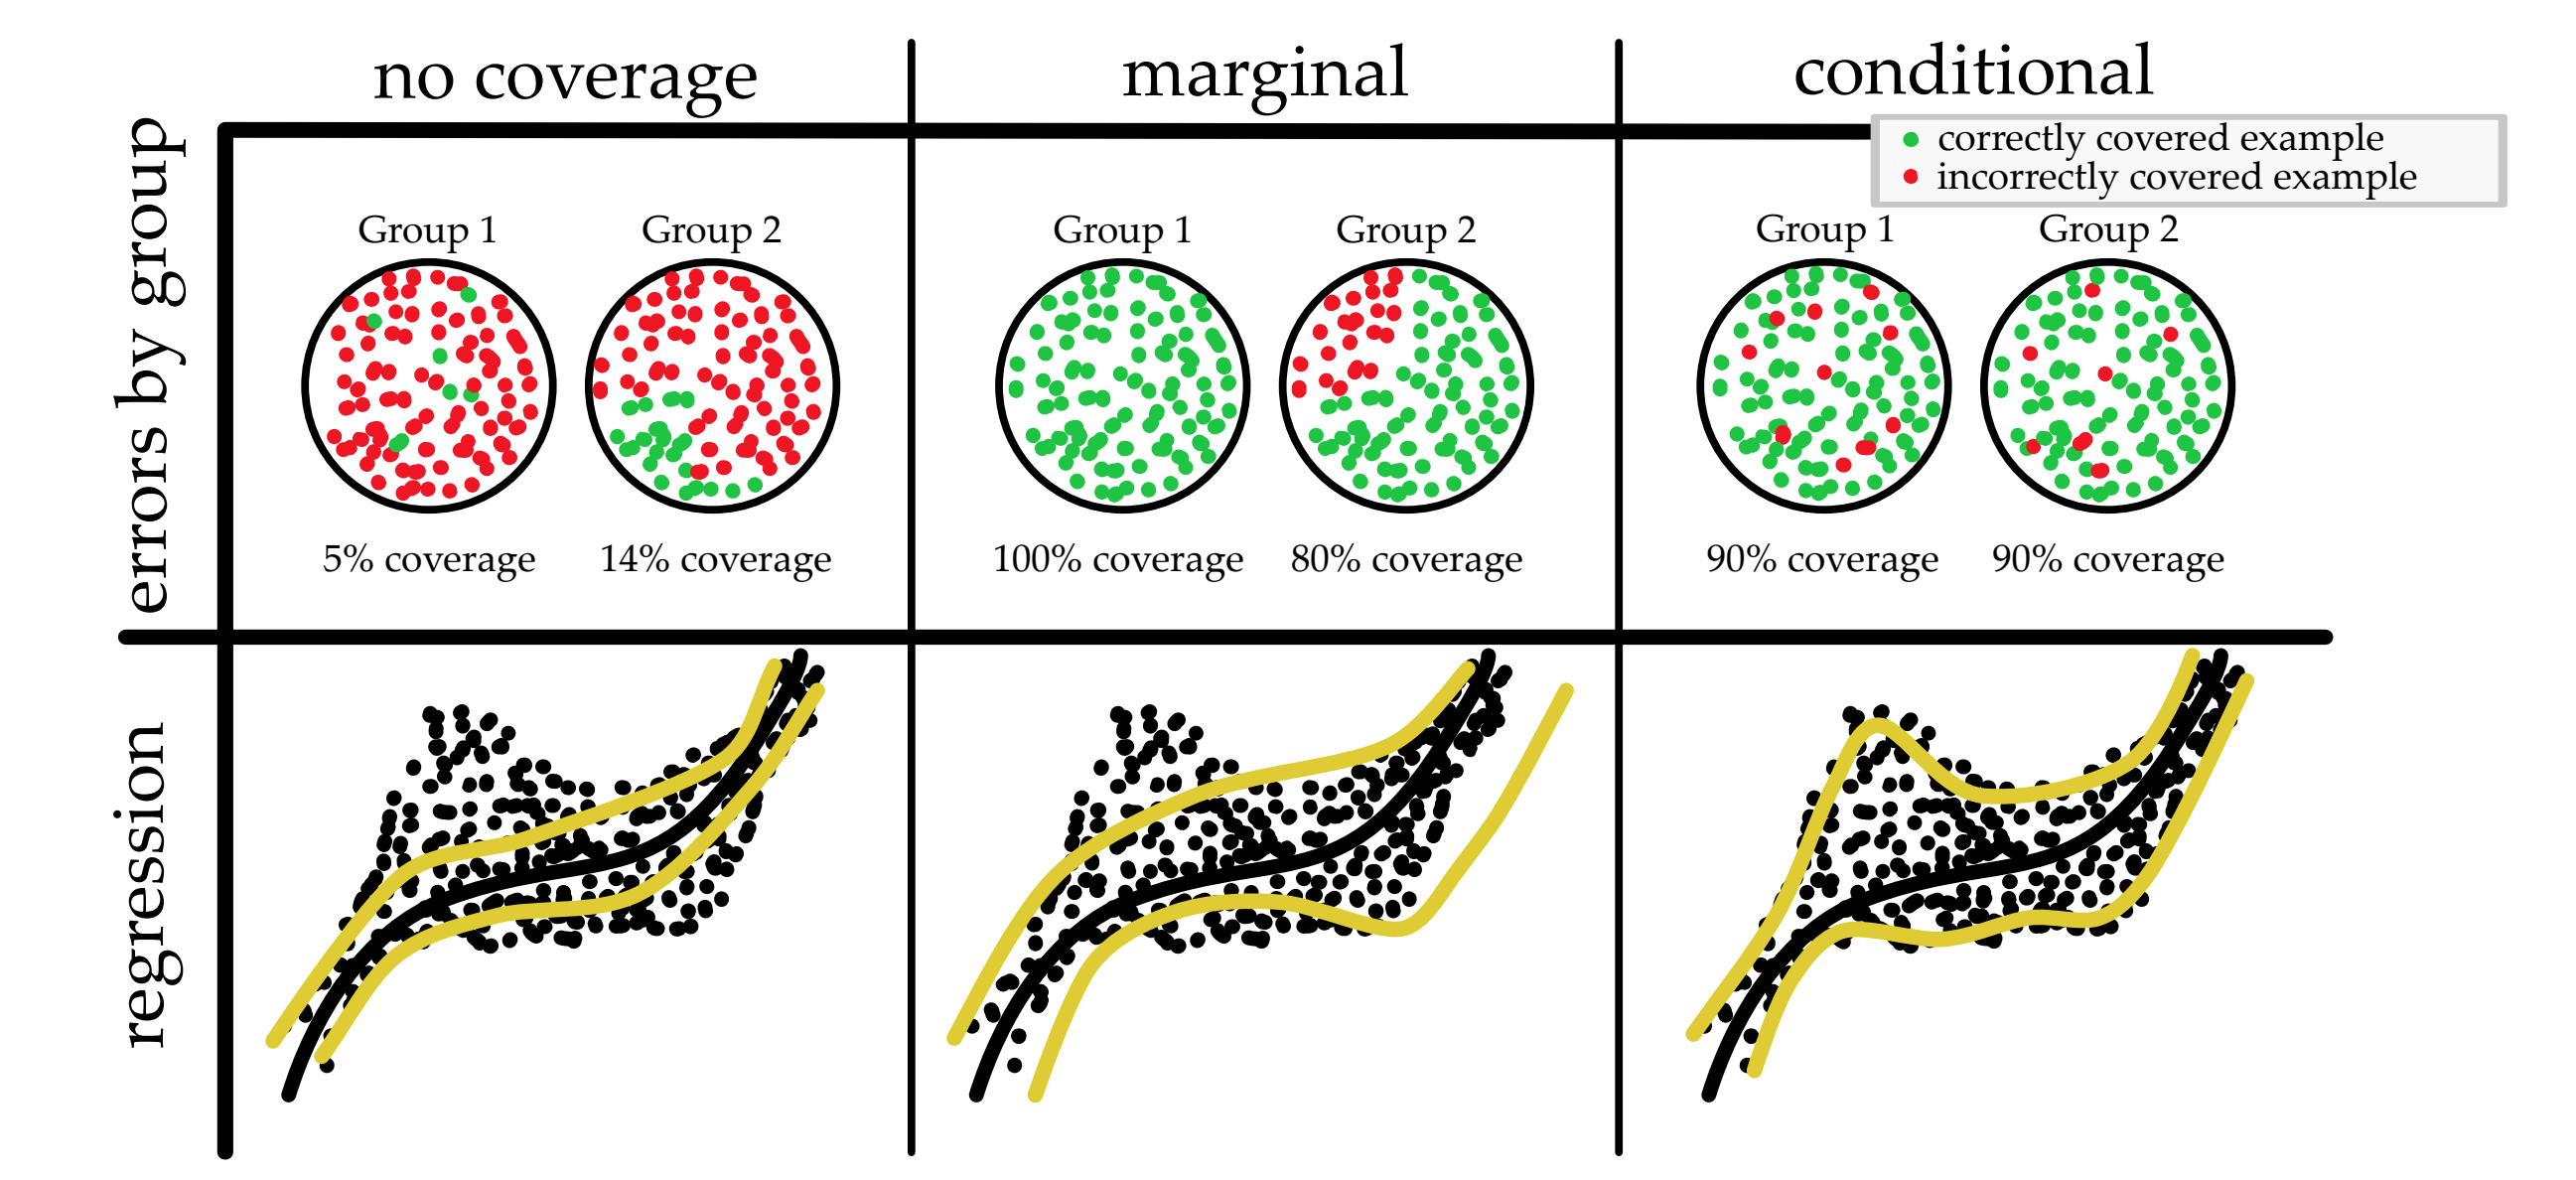
\includegraphics[width=\textwidth]{capitulos/cap_02/imagenes/coverage_types.png}
    \caption[
        Esquema gráfico de conjuntos de predicción bajo distintas nociones de cobertura: sin cobertura garantizada, con cobertura marginal y con cobertura condicional. 
    ]{
        Esquema gráfico de conjuntos de predicción bajo distintas nociones de cobertura: sin cobertura garantizada, con cobertura marginal y con cobertura condicional. Recuperado de \cite{angelopoulos2021}.
        %
        En la parte inferior de la figura se muestra la amplitud de los intervalos de predicción (en línea amarilla) generados en un problema de regresión. En la parte superior, las instancias se dividen en dos grupos; los valores reales contenidos en los intervalos se representan en verde, mientras que los no contenidos aparecen en rojo.
        %
        La primera columna ilustra un caso con intervalos de predicción demasiado estrechos, lo que resulta en una baja cobertura: la mayoría de los valores reales quedan fuera del intervalo.
        %
        En la segunda columna, los intervalos son más amplios y permiten capturar una mayor proporción de los valores reales, alcanzando una cobertura marginal del 90\% en el conjunto total. Sin embargo, esta cobertura no se distribuye equitativamente: el error se concentra en una región específica dentro de uno de los grupos, lo que indica ausencia de cobertura condicional.
        %
        Finalmente, en la tercera columna, los intervalos se ajustan a la distribución de las predicciones, logrando cobertura marginal como condicional del 90\%, con un error repartido de manera uniforme entre regiones y grupos, reflejando una calibración más precisa y equitativa del modelo.
    } 
    \label{fig:coverage}
\end{figure}


Además, el conjunto de calibración debe ser estadísticamente representativo de la distribución completa de los datos. Esto crea un compromiso fundamental: asignar más ejemplos a la calibración mejora la precisión de los intervalos predictivos, pero a costa de reducir el tamaño del conjunto de entrenamiento, lo que potencialmente puede empeorar el rendimiento del modelo base.

Algunas características deseables en las técnicas de \acrshort{CP} son:

\begin{itemize}
    \item \textbf{Independencia del modelo (\textit{model-agnostic})}: que no requiera reentrenar el modelo ni modificar su arquitectura, permitiendo su aplicación \textit{post-hoc} a modelos preentrenados.

    \item \textbf{Independencia del dominio (\textit{domain-agnostic})}: que pueda manejar entradas de cualquier tipo sin restricciones, tantos datos estructurado como no estructurados. En este trabajos todos los métodos estudiados presentan esta característica.
     
    \item \textbf{Predicción adaptativa (\textit{adaptive prediction})}: se refiere a que el intervalo o conjunto de predicción varía su tamaño en función de la incertidumbre asociada a cada predicción individual. En general, cuanto más rica y específica sea la información que la técnica utiliza sobre las predicciones y su incertidumbre, más adaptativa será la predicción conformal.
    Esta adaptatividad aproxima a la cobertura condicional.

    \item \textbf{Ser eficiente computacionalmente}: es deseable que tanto la fase de calibración como la inferencia sean rápidas y no introduzcan una sobrecarga significativa en comparación con la predicción puntual.
    
    Aunque la mayoría de los métodos de predicción conformal presentan una sobrecarga computacional moderada, esta puede variar dependiendo del enfoque utilizado. Por ejemplo, las técnicas basadas en \textit{split conformal} ---las únicas que exploraremos en este trabajo--- suelen ser más eficientes que aquellas que requieren reentrenamiento múltiple, como en algunos métodos \textit{Cross conformal prediction} o \textit{Jackknife+}%
    \footnote{
        \textit{Cross conformal prediction} \cite{vovk2015} y \textit{Jacknife+} \cite{barber2021} son métodos de \acrshort{CP} que mejoran las garantías de cobertura de técnicas de \acrshort{CP} mediante el uso más eficiente de los datos disponibles para calibración y entrenamiento, de forma análoga a la validación cruzada (\textit{cross-validation}) o el \textit{leave-one-out}, respectivamente.
    }.
    
    % \item \textbf{Robustez frente a datos ruidosos y detección de datos \textit{out-of-distribution}}%
    % \footnote{
    %     Los datos \textit{out-of-distribution} son datos que no provienen de la misma distribución que los datos con los que se entrenó el modelo.
    % }:
    % que los intervalos reflejen adecuadamente la incertidumbre ante datos corruptos o fuera del dominio de entrenamiento, ya sea detectando de que el dato es anómalo o dando un intervalo/conjunto de predicción muy amplio. 

\end{itemize}

% En general, existe un \textit{trade-off} entre flexibilidad y precisión: las técnicas dependientes del modelo, del dominio o incluso del propio problema (p.ej., incluyendo información experta), que asumen ciertas distribuciones de los datos, pueden cuantificar mejor la incertidumbre aleatoria y epistémica, y producir intervalos más ajustados e informativos. 

% \todo{Este último párrafo es una valoración que yo he realizado muy priori}


% ------------------------------------------------------------------------------------------------------------

\subsection{Algoritmo conformal}

Existen multitud de técnicas de \acrshort{CP}. Generalmente, estas dependen del tipo de problema a resolver: regresión \cite{papadopoulos2002, romano2019, bethell2024}, clasificación \cite{sadinle2019, romano2020, angelopoulos2020}, series temporales \cite{xu2021, zaffran2022, stankeviciute2021}%
\footnote{
    El marco de \acrshort{CP} clásico asume que los datos son intercambiables, una propiedad que no se cumple en las series temporales debido a la dependencia secuencial entre observaciones. A pesar de ello, se han desarrollado diversas extensiones del enfoque conformal para adaptarse a estos datos.
},
o detección de anomalías \cite{laxhammar2015}, entre otros. 
A pesar de su diversidad, todos los algoritmos conformales comparten un elemento clave: la definición de una 
\textbf{función de no conformidad} $NC(x_i,y_i)$, una heurística que mide la incertidumbre asociada a cada predicción. Intuitivamente, esta función actúa como una medida de discrepancia entre el valor predicho y el valor observado, y permite determinar cuán ``extraña'' o ``no conforme'' es una nueva observación respecto al comportamiento esperado del modelo.

La implementación de la predicción conformal consta de los siguientes pasos:

\begin{enumerate}

    \item Se divide el conjunto de datos disponible en dos subconjuntos: un conjunto de entrenamiento, utilizado para ajustar el modelo predictivo ---es decir, para entrenar el modelo de forma habitual---, y un conjunto de calibración, que se reserva exclusivamente para estimar la incertidumbre mediante el cálculo de las puntuaciones de no conformidad. Esta separación permite que la estimación del intervalo de predicción sea independiente del proceso de entrenamiento, lo cual es crucial para garantizar la validez estadística del método.

    \item Se entrena el modelo predictivo con los ejemplos del conjunto de entrenamiento. 

    \item \textbf{Calibración conformal}: En este, se calculan las \textbf{puntuaciones de no conformidad (\textit{nonconformity scores}) $R$}%
    \footnote{
        En la literatura, a este vector de puntuaciones se le suele denotar como $R$ por \textit{`residual'}
        o $E$ por \textit{`error'}. 
    }:

    $$
    R = \left\{ NC(x_i,y_i) \right\}_{i=1}^n
    $$

    donde $n$ es el número de ejemplos del conjunto de calibración.

    Estas puntuaciones se derivan a partir de una heurística que combina al menos el valor real y el predicho del problema con otras posibles fuentes de información, como las propias entradas o incluso representaciones internas del modelo%
    \footnote{
        Cabe señalar que una técnica será independiente del modelo y del dominio cuando solo tenga en cuenta las salidas del modelo y los valores reales del problema para realizar la \acrshort{CP}.
    }. 
    Bajo las garantías estadísticas que ofrece el marco teórico de la \acrshort{CP}, esta flexibilidad muestra un gran potencial para ser integrada con otras técnicas de \acrshort{UQ}, ampliando así sus aplicaciones y mejorando la robustez de las estimaciones de incertidumbre.

    Independientemente del diseño específico de la función de no conformidad, esta debe cumplir una condición esencial: las puntuaciones deben ser intercambiables entre el conjunto de calibración y las nuevas instancias. En otras palabras, deben ser idénticamente distribuidas. Esta propiedad es crucial para que \acrshort{CP} garantice cobertura marginal válida a un nivel de confianza determinado. Por tanto, aunque existe flexibilidad en el diseño de la función de no conformidad, su elección debe considerar tanto la capacidad para capturar incertidumbre útil como el cumplimiento del supuesto de intercambiabilidad. 

    A continuación, se calcula el \textbf{umbral de no conformidad}. Para un nivel de significación$\alpha$, se selecciona el $(1 - \alpha)(1 + 1/n)$-ésimo cuantil%
    \footnote{
        La corrección $(1 + 1/n)$ asegura validez estadística para conjuntos de tamaño finito.
    } 
    de las puntuaciones de no conformidad obtenidas en el conjunto de calibración (véase la Figura \ref{fig:nonconformity_quantile_comparison}).

    $$
    \delta_\alpha = Quantile_{ \lceil  (1-\alpha) (1 + 1/n)  \rceil } ( \left\{ NC(x_i,y_i) \right\}_{i=1}^n )
    $$

    \begin{figure}[htbp]
        \centering

        \begin{subfigure}[b]{0.48\textwidth}
            \centering
            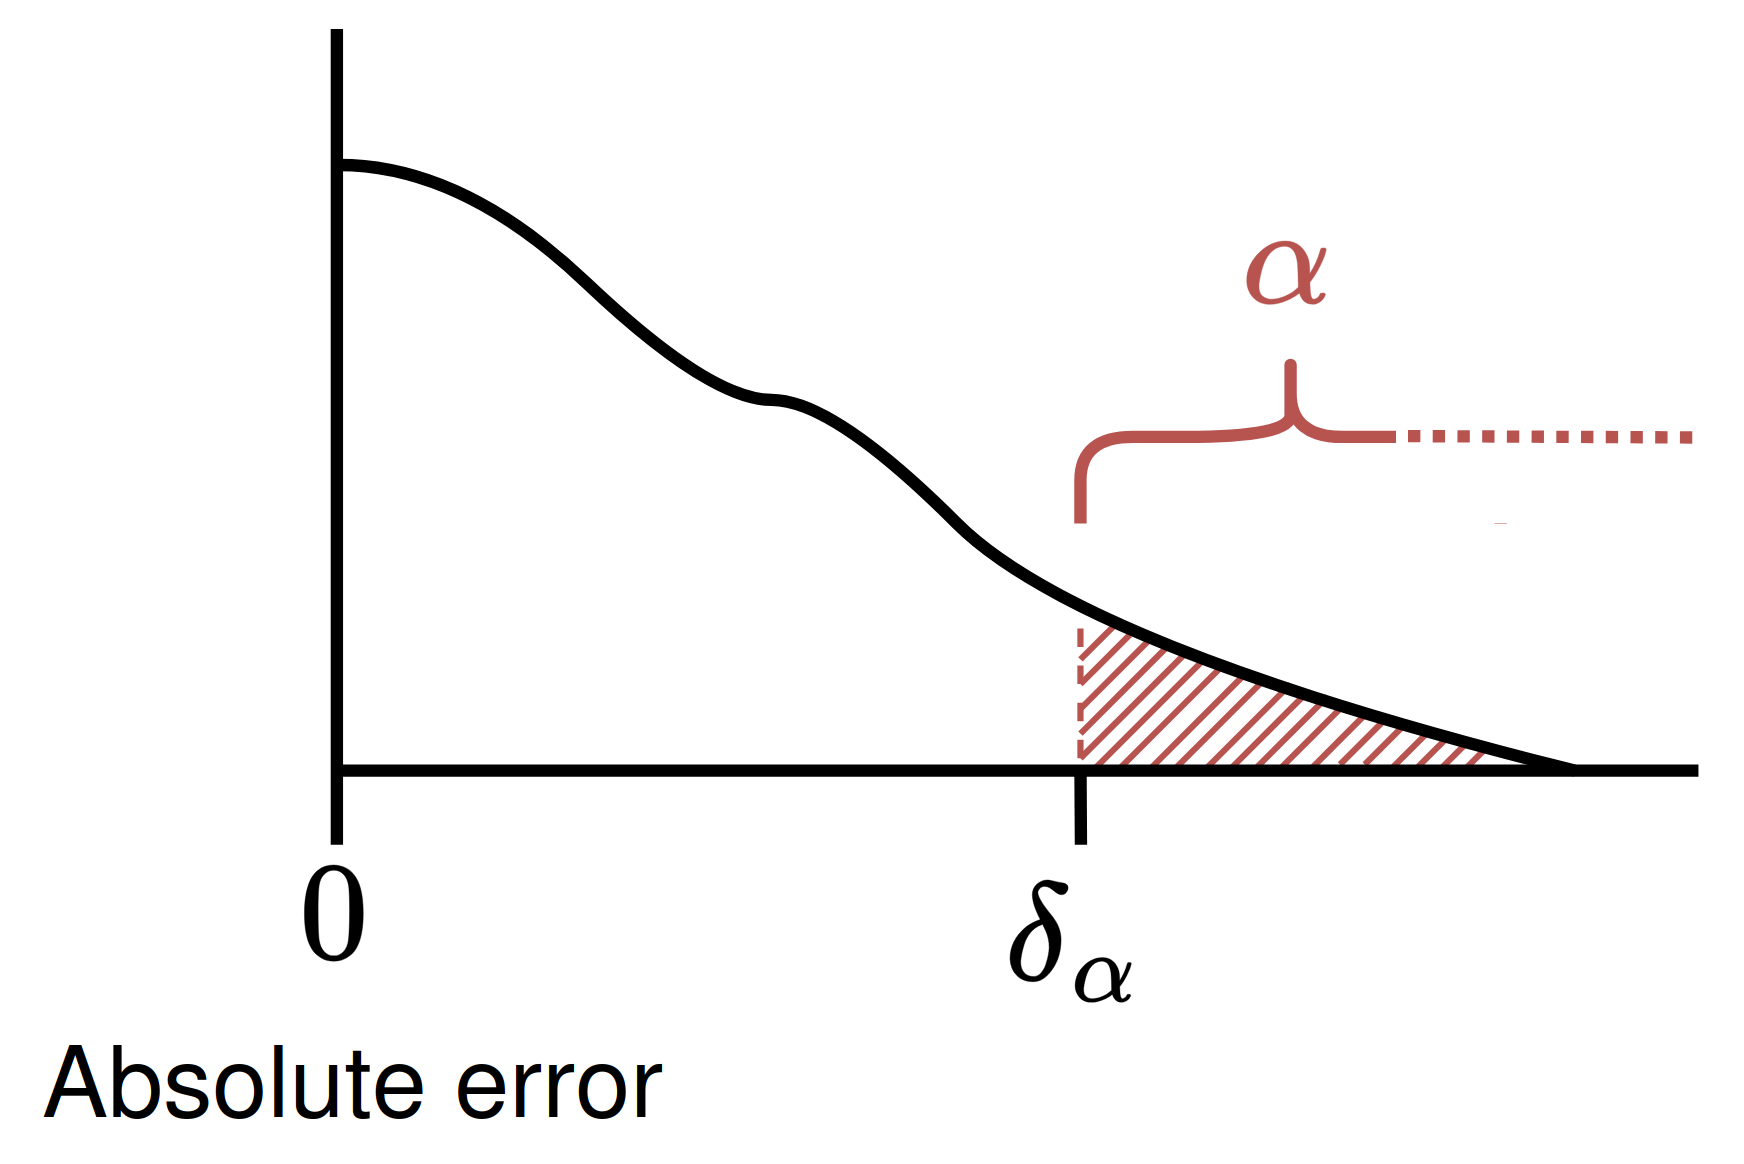
\includegraphics[width=\textwidth]{capitulos/cap_02/imagenes/nonconformity_quantile_threshold_simetric.png}
            \caption{Intervalos simétricos.}
            \label{fig:nonconformity_quantile_threshold_simetric}
        \end{subfigure}
        \hfill
        \begin{subfigure}[b]{0.49\textwidth}
            \centering
            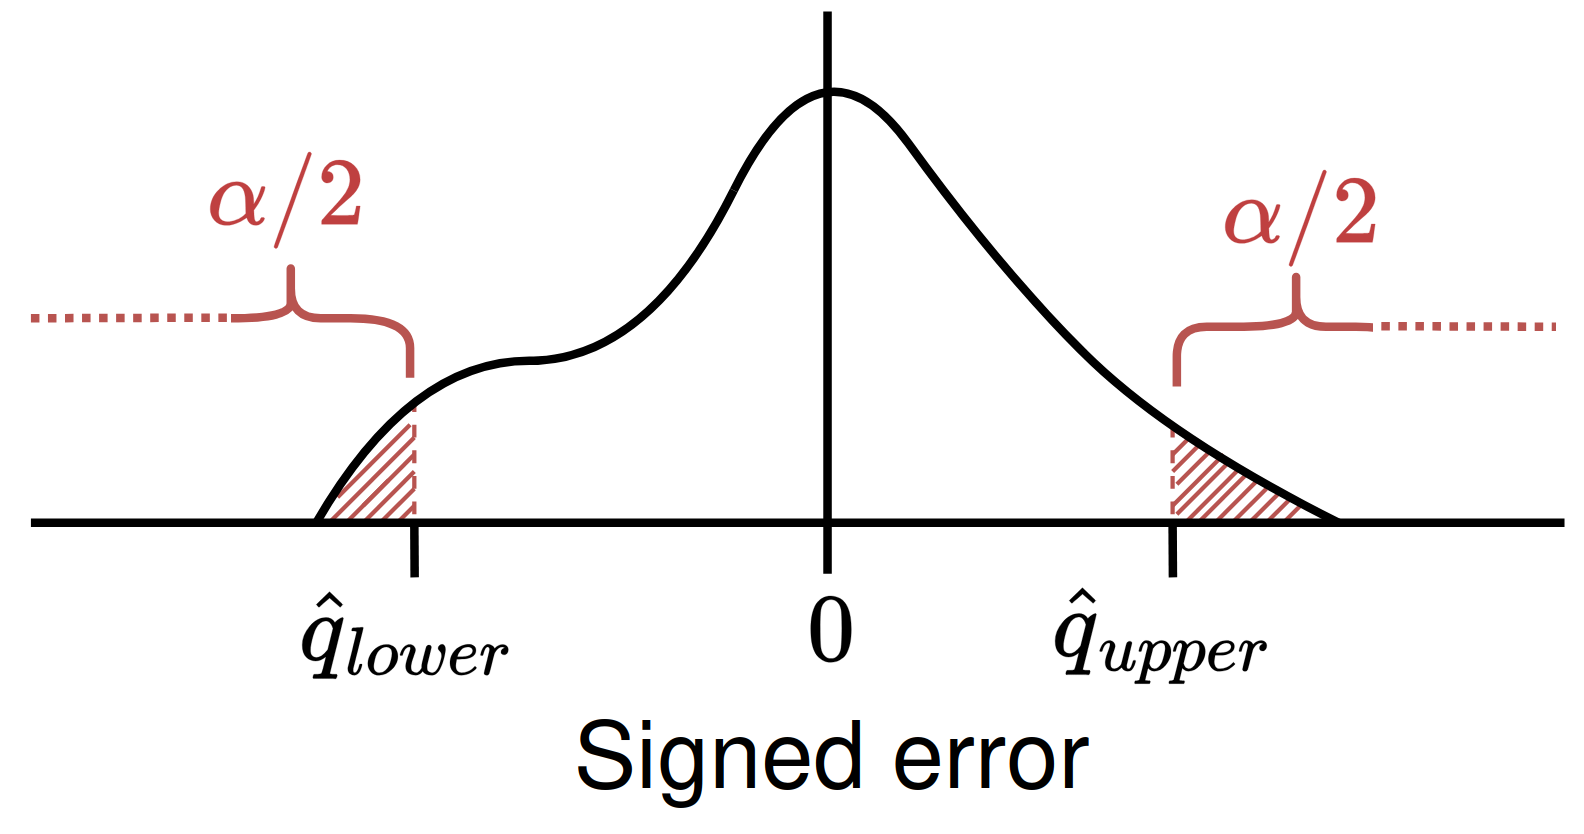
\includegraphics[width=\textwidth]{capitulos/cap_02/imagenes/nonconformity_quantile_threshold_asimetric.png}
            \caption{Intervalos asimétricos.}
            \label{fig:nonconformity_quantile_threshold_asimetric}
        \end{subfigure}

        \caption[
            Determinación del umbral de no conformidad para intervalos simétricos y asimétricos.
        ]{
            Determinación del umbral de no conformidad para intervalos simétricos y asimétricos. 
            En (\ref{sub@fig:nonconformity_quantile_threshold_simetric}), el error es absoluto, y el umbral
            se calcula como se ha especificado anteriormente. 
            En (\ref{sub@fig:nonconformity_quantile_threshold_asimetric}), el error tiene signo, y hay dos
            umbrales de incertidumbre, uno por cada cola, calculado como el cuantil con significación
            $\alpha/2$ de los errores negativos y de los errores positivos, respectivamente para el umbral
            inferior y el umbral superior. 
        }
        \label{fig:nonconformity_quantile_comparison}
    \end{figure}


    \item \textbf{Inferencia conformal}: Para cada nueva instancia $x_{n+1}$ se genera una predicción puntual
    $y_{n+1}$ utilizando el modelo entrenado. Luego, se construye un conjunto o intervalo de predicción
    $\Gamma(x_{n+1})$ a partir de la predicción puntual y el umbral de no conformidad $\hat{q}_{1-\alpha}$, 
    tal que se garantiza con nivel de confianza $1-\alpha$ que el verdadero valor $y_{n+1}$ pertenezca al
    conjunto:
    
    $$
    y_{n+1} \in \Gamma_{1-\alpha}(x_{n+1})
    $$

    La forma de construir $\Gamma(x_{n+1})$ depende de cómo se haya definido la función de no conformidad 
    durante la fase de calibración.

\end{enumerate}




Por ejemplo, en la técnica \textit{Inductive Conformal Prediction} \cite{papadopoulos2002} para problemas de regresión, ---que describiremos en mayor profundidad en el Capítulo 4---, se utiliza el error absoluto como función de no conformidad:

$$
NC(x_i, y_i) = | y_i - \hat{f}(x_i) |
$$

El umbral de no conformidad se obtiene como el $(1 - \alpha)(1 + 1/n)$-ésimo cuantil de las puntuaciones de no conformidad (véase la Figura \ref{fig:nonconformity_quantile_threshold_simetric}):

$$
\delta_\alpha = Quantile_{ \lceil  (1-\alpha) (1 + 1/n)  \rceil } ( \left\{ NC(x_i,y_i) \right\}_{i=1}^n )
$$

La construcción del intervalo de predicción surge directamente de despejar el valor real $y_{n+1}$ en la expresión que iguala la función de no conformidad, evaluada sobre la nueva instancia, con el umbral de no conformidad. En este caso en el que se emplea el error absoluto, es decir:

$$
NC(x_i, y_i) = | y_i - \hat{f}(x_i) |
$$

entonces al imponer la condición $NC(x_{n+1}, y_{n+1}) \le \delta_\alpha$, se obtiene: 

$$
|y_{n+1}-\hat{f}(x_{n+1})| \le \delta_\alpha
$$

Despejando $y_{n+1}$, se obtiene:

$$
\hat{f}(x_{n+1}) - \delta_\alpha \le y_{n+1} \le \hat{f}(x_{n+1}) + \delta_\alpha 
$$

Por tanto, el intervalo de predicción conformal está dado por:

$$
y_{n+1} \in \left[ \hat{f}(x_{n+1})-\delta_\alpha , \hat{f}(x_{n+1})+\delta_\alpha  \right] 
$$

Esta expresión determina los límites inferior y superior del intervalo de predicción conformal para dicha
instancia.


A continuación se presenta un ejemplo numérico para ilustrar la construcción del intervalo. Supongamos que $x_i$ es un vector de unos determinados indicadores osteológicos de un individuo con edad cronológica conocida $y_i$ (en años). Entrenamos un modelo de regresión $\hat{f}$ en un conjunto de entrenamiento y reservamos un conjunto de calibración de $n$ individuos identificados.
Se supone un conjunto de calibración de $n=50$ individuos y $\alpha=0.10$. Calculamos los residuos absolutos $NC(x_i,y_i)$ en calibración y obtenemos su cuantil, $(1-\alpha)(1+1/n)=0.90\times1.02=0.918$ (percentil $91.8$). Si ese cuantil es $\delta_{0.10}=3.3$ años y para un caso nuevo $\hat{f}(x_{n+1})=34.7$ años, entonces:

$$
y_{n+1} \in \left[ 34.7 - 3.3 , 34.7 + 3.3  \right] = \left[ 31.4 , 38.0 \right] \textnormal{ años}
$$

